\documentclass[11pt]{article}

\usepackage[T1]{fontenc}
\usepackage[margin=1in]{geometry}
\usepackage{amsmath,amssymb,mathtools,bm}
\usepackage{booktabs,longtable,tabularx,array}
\usepackage{enumitem}
\usepackage{graphicx}
\usepackage{placeins}
\usepackage{xcolor}
\usepackage{hyperref}
\usepackage{microtype}

\hypersetup{
  colorlinks=true,
  linkcolor=blue!45!black,
  citecolor=blue!45!black,
  urlcolor=blue!45!black
}

\setlength{\emergencystretch}{3em}
\setlist[itemize]{topsep=3pt,itemsep=2pt}
\setlist[enumerate]{topsep=3pt,itemsep=3pt}

\newcommand{\T}{\mathbb T}
\newcommand{\R}{\mathbb R}
\newcommand{\G}{\mathcal G}
\newcommand{\dd}{\,\mathrm d}
\newcommand{\norm}[1]{\left\lVert #1\right\rVert}
\newcommand{\eps}{\varepsilon}

\title{A Parameterized Training Corpus for the\\
Dirichlet--Neumann Operator\\[0.4em]
\large Design, implementation checks, and direct comparison with
\texttt{combined\_dataset\_v9}}
\author{}
\date{27 July 2026}

\begin{document}
\maketitle

\begin{abstract}
The historical training archive for the periodic Dirichlet--Neumann operator
combines generators with different sampling, filtering, target, and snapshot
rules.  It is therefore difficult to separate the effects of physical
coverage, numerical labels, and source-dependent row counts.

This document specifies a prospective replacement corpus with four physical
families: fifth-order Stokes states, periodic Tanaka profiles,
Benjamin--Feir sideband states, and resolved-band JONSWAP/TMA random seas.
All four use one discrete order-six DNO target, case-level splitting, equal
case weight, and reproducible case records.  The three trajectory families
use one residual-controlled two-stage, fourth-order Gauss--Legendre
calculation with step \(0.01\); a case is retained only when that calculation
returns a complete admissible trajectory.  Static Stokes cases instead
require a finite state in the declared Stokes support.  Airy,
manufactured-DNO, and sparse-Fourier cases are reserved for validation.

The four samplers, constructors, common target, one-arm trajectory executor,
bounded accepted-case scheduler, restart records, combined dataset view, and
case-balanced loader are implemented and pass focused CPU tests.  The corpus
itself has not been generated.  Its remaining numerical gate is an
exact-contract GPU calculation that obtains one accepted case from each
trajectory parameter category.
\end{abstract}

\tableofcontents
\clearpage

\noindent\textit{Reading guide.}
The document proceeds from the DNO target to the four initial-condition
formulas, reference rollouts, whole-case acceptance, and balanced training
batches.
Sections~\ref{sec:dataset-design}, \ref{sec:target}, \ref{sec:families},
\ref{sec:acceptance}, and \ref{sec:splitting} define that chain.  The
difference from the historical archive and the work remaining before
generation are stated separately.  The
detailed \texttt{v9} audit is in Appendix~\ref{sec:v9}.

\section*{Implementation status}

The replacement corpus itself has not yet been generated.  The following
table distinguishes implemented definitions and tests from the one remaining
pre-generation calculation:
\begin{center}
\small
\begin{tabularx}{\textwidth}{
  @{}>{\raggedright\arraybackslash}p{0.20\textwidth}
     >{\raggedright\arraybackslash}p{0.18\textwidth}
     >{\raggedright\arraybackslash}X@{}}
  \toprule
  Item & Status & Evidence \\
  \midrule
  Discrete target
    & Frozen
    & $L=2\pi$, $g=1$, order six, $N=1024$, pad factor eight, and delivered band
      $|k|\leq128$; fixed-band, mean, translation, and dtype tests pass. \\
  Finite-depth Stokes
    & Exact bounded path passed
    & The four-category sampler enforces the conservative condition
      $\mathrm{Ur}_+\leq26$.  At
      $(N,M,p,K)=(1024,6,8,128)$, one revision-2 case per category passed
      the complete sampled-specification, construction, target, quality,
      archive, and dataset-view transaction through the bounded quota
      executor.  The loader returns four finite one-row cases. \\
  Tanaka
    & Sampler, constructor, and quota path implemented
    & The eleven-category direction-aware periodic-gap sampler and
      tangent-Hermite constructor are
      connected to the common transaction.  Only a finite negative potential
      radicand is outside the declared construction; nonfinite algebra or an
      invalid wave speed stops generation.  A reduced revision-1 wiring smoke
      reached the dataset loader. \\
  Benjamin--Feir
    & Sampler and quota path implemented
    & The 66 admissible integer pairs are parameter categories.  Conditional
      steepness, amplitude ratio, and phase sampling are connected through a
      durable attempt record to the equation-(33) constructor and common
      trajectory transaction.  A reduced revision-1 wiring smoke reached the
      dataset loader. \\
  Random sea
    & Sampler and quota path implemented
    & The 27 declared categories have continuous parameter laws and stored
      phase arrays.  A reduced revision-1 wiring smoke passed through the
      durable transaction and dataset view. \\
  Common trajectory transaction
    & Implemented
    & One float64 rollout with GL2 step $0.01$, saved spacing $0.08$, stage
      residual telemetry, post-acceptance time selection, a complete-case
      writer, and a split-aware loader are executable and tested.  The
      $0.01/0.005$ pair remains a validation calculation and is not run for
      each production case. \\
  Accepted-quota recovery
    & Bounded run specification implemented
    & The driver reconstructs checked accepted counts, replays proposal-only
      and proposal-plus-shard transaction states, and admits one writer.  A
      category requesting $Q_i$ accepted cases has at most $4Q_i$ durable
      attempts.  Pending work at the ceiling is replayed; a resolved
      deficient category at the ceiling terminates the family run instead of
      silently changing its population. \\
  Combined view and loader
    & Implemented
    & The view verifies transaction hashes without copying field arrays.
      In each training epoch the loader selects one stored time from every
      accepted case; validation uses one fixed time per case. \\
  Time-step validation
    & Fixed diagnostic panel complete
    & Ten complete cases agree between GL2 steps $0.01$ and $0.005$ to at
      most $1.126337\times10^{-5}$.  The steep Tanaka and equation-(33)
      Benjamin--Feir calculations become incomplete at nearly the same
      physical times under both steps.  The comparison supports the
      production step $0.01$; it is not a production rejection filter. \\
  Generation gate
    & GPU calculation running
    & A prior generator-revision-1 paired-step four-family smoke accepted one
      case per family and assembled 417 finite rows.  The revision-2
      104-category gate is running.  Bulk generation still waits for it to
      obtain a single-arm production case from each of the 11 Tanaka, 66
      Benjamin--Feir, and 27 random-sea parameter categories under the final
      bounded scheduler. \\
  \bottomrule
\end{tabularx}
\end{center}

\section{Dataset organization}
\label{sec:dataset-design}

Let $L>0$ be the horizontal period and
$\T_L=\R/(L\mathbb Z)$ the periodic interval, with horizontal coordinate
$x\in\T_L$.  Each training case stores a real surface elevation
$\eta_0(x)$, a real surface-potential trace $\xi_0(x)$, and a constant mean
depth $h>0$.  It also stores whether it was generated as a Stokes, Tanaka,
Benjamin--Feir, or random-sea case and every numerical parameter required to
reconstruct that initial state.  The four constructions are defined
explicitly in Section~\ref{sec:families}.
Every accepted initial state satisfies
\begin{equation}
  \int_{\T_L}\xi_0(x)\,\dd x=0,
  \qquad
  \min_{x\in\T_L}\{h+\eta_0(x)\}>0.
  \label{eq:case-gauge-and-depth}
\end{equation}
The first condition fixes the irrelevant additive constant in $\xi_0$; the
second excludes an initial dry point.  Depth is stored with the case and held
fixed during a rollout.

The dataset rules are:
\begin{enumerate}
  \item Generate the same accepted case count from each family.  Balance
        the coarse parameter ranges listed in Section~\ref{sec:families}.
  \item First require the sampled specification to lie in its declared
        family support and its declared constructor to return a well-defined
        periodic initial state.  For Tanaka cases specifically, a finite
        negative radicand is outside the declared construction; a nonfinite
        radicand or an invalid wave speed stops generation.  The trajectory
        adapters also require the assembled initial arrays to be finite, the
        depth to be positive, and \(h+\eta_0>0\) on the grid.  Failure of
        these constructor invariants stops generation rather than becoming
        an ordinary zero-row draw.  For a trajectory
        family, retain the complete case only if the single fixed-step
        calculation produces a complete admissible numerical trajectory as
        defined in Section~\ref{sec:acceptance}; static Stokes cases retain
        one well-defined state in their declared support.  A failed
        trajectory contributes zero frames.
  \item At each training epoch, choose one stored time uniformly from every
        accepted training case and then batch the selected rows.  Because the
        accepted case count is the same in all four families, every family and
        every case has equal epoch weight.  Validation uses one fixed,
        deterministic stored time from every validation case.
  \item Keep Airy, manufactured-DNO, and sparse-Fourier cases out of training.
        They are diagnostic tests only.
\end{enumerate}
There is no production rejection rule based on sign changes, slope, extrema,
Hamiltonian drift, absolute target size, or visual appearance.
The replacement corpus uses low-steepness Stokes states instead of a separate
single-mode family, and a standard finite-depth random-sea spectrum instead
of the old Gaussian sea.  Its shallow mixed-mode coverage is tested as
specified in Section~\ref{sec:execution}.  The existing \texttt{v9} archive
remains the experimental baseline.

\section{Learning problem and discrete target}
\label{sec:target}

Let $g>0$ denote gravitational acceleration; the generated corpus uses the
nondimensional value $g=1$.  For each integer Fourier index $n$, define the
wavenumber $k_n=2\pi n/L$.  For any integrable $L$-periodic function $u$, use
the Fourier convention
\begin{equation}
  \widehat u_n=\frac1L\int_{\T_L}u(x)e^{-ik_nx}\,\dd x,
  \qquad
  u(x)=\sum_{n\in\mathbb Z}\widehat u_ne^{ik_nx}.
  \label{eq:fourier-convention}
\end{equation}
For an $N$-point grid, define the spacing $\Delta x=L/N$ and nodes
$x_j=j\Delta x$ for $j=0,\ldots,N-1$.  The normalized continuous and grid
norms are
\begin{equation}
  \norm{u}_{2,L}^2=\frac1L\int_{\T_L}|u|^2\,\dd x,
  \qquad
  \norm{u}_{2,N}^2=\frac1N\sum_{j=0}^{N-1}|u(x_j)|^2.
  \label{eq:l2-conventions}
\end{equation}
Unless a subscript is shown, $\norm{\cdot}_2$ means the corresponding
normalized norm on the representation being discussed.  Fix a maximum
retained wavenumber $K>0$.  Let $P_K$ be the fixed-band projection, let
$\mathcal J_K$ be the set of its retained positive Fourier indices, and let
the indicator $\mathbf 1_{\{\cdot\}}$ equal one when the condition in braces
holds and zero otherwise:
\begin{equation}
  \widehat{P_Ku}_n=\mathbf 1_{\{|k_n|\leq K\}}\widehat u_n,
  \qquad
  \mathcal J_K=\{n\in\mathbb Z:n\geq1,\ k_n\leq K\}.
  \label{eq:fixed-band-projection}
\end{equation}
The projection acts componentwise when its argument is an ordered pair of
fields.
Define the mean-removal operator $P_0^\perp$ and the mean-zero band
projection $P_K^\circ$ by
\begin{equation}
  P_0^\perp u=u-\widehat u_0,\qquad
  P_K^\circ=P_0^\perp P_K.
  \label{eq:mean-zero-band-projection}
\end{equation}
Thus $P_K^\circ$ both restricts the band and fixes the zero-mean gauge.  It is
used for DNO outputs and for the $\xi$ component of the vector field; $P_K$
alone is used for $\eta$, whose mean is the conserved mass.
The frozen target cutoff is $K=128$, and the random-sea transition begins at
$K_0=96$.  For a nonnegative wavenumber $k$, the random-sea formula uses the
separate smooth window
\begin{equation}
  W_{K,K_0}(k)=
  \begin{cases}
    1,&0\leq k\leq K_0,\\
    \cos^2\!\left[\dfrac{\pi}{2}\dfrac{k-K_0}{K-K_0}\right],
      &K_0<k<K,\\
    0,&k\geq K.
  \end{cases}
  \label{eq:resolved-band-window}
\end{equation}
Unlike $P_K$, this window changes the constructed initial condition; the two
operations must not be conflated.  We write $W_K:=W_{K,K_0}$ for the frozen
choice $(K_0,K)=(96,128)$.

For a surface elevation $\eta(x)$ and depth $h>0$, let $y$ denote the vertical
coordinate and define the fluid domain
\begin{equation}
  \Omega_{\eta,h}
  =\{(x,y):x\in\T_L,\ -h<y<\eta(x)\}.
\end{equation}
For surface Dirichlet data $\xi$, let $\varphi$ solve
\begin{equation}
  \Delta\varphi=0\quad\text{in }\Omega_{\eta,h},\qquad
  \varphi_y(x,-h)=0,\qquad
  \varphi(x,\eta(x))=\xi(x).
\end{equation}
The physical Dirichlet--Neumann operator is
\begin{equation}
  G(\eta;h)\xi
  =\left(\varphi_y-\eta_x\varphi_x\right)_{y=\eta(x)}.
  \label{eq:physical-dno}
\end{equation}
Let $D=-i\partial_x$, so $|D|$ is the Fourier multiplier with symbol
$|k_n|$.  For each integer $m\geq0$, let $G_m$ be the Craig--Sulem term
homogeneous of degree $m$ in $\eta$, and let $M$ be the largest retained
order.  The current solver uses
\begin{equation}
  G_M(\eta;h)\xi=\sum_{m=0}^{M}G_m(\eta;h)\xi,\qquad
  G_0(h)=|D|\tanh(h|D|).
  \label{eq:cs-truncation}
\end{equation}
In particular,
\begin{equation}
  G_1(\eta;h)\xi
  =-G_0(h)\!\left(\eta G_0(h)\xi\right)
   -\partial_x\!\left(\eta\,\partial_x\xi\right).
  \label{eq:first-cs-term}
\end{equation}
This formula fixes the meaning of the analytic $G_0+G_1$ backbone referenced
later in the diagnostic discussion.

We distinguish the physical operator in \eqref{eq:physical-dno} from its
fully discrete evaluation.  Let $\G^{N,p}_M$ denote the order-$M$
pseudospectral recursion on $N$ points with padding factor $p$.  The frozen
common learning target is
\begin{equation}
  \boxed{
  G_{\mathrm{ref}}(\eta;h)\xi
  =P_K^\circ\!\left[
    \G^{N,p}_M(P_K\eta;h)(P_K\xi)
  \right].}
  \label{eq:common-target}
\end{equation}
The frozen paper target uses
\begin{equation}
  L=2\pi,\qquad g=1,\qquad M=6,\qquad
  N=1024,\qquad p=8,\qquad K=128.
  \label{eq:candidate-discretization}
\end{equation}
The evaluation in \eqref{eq:common-target} is performed in float64 and only
the final arrays are stored in float32.  Statements that a constructed field
has zero mean refer to the float64 value before storage; float32 conversion
preserves the condition only to rounding error.

Equation \eqref{eq:common-target} says exactly which discrete formula the model is
trained to reproduce.  A claim that this formula approximates the physical $G$
requires separate convergence evidence in $M$, $N$, and $p$.  Fixed-$M$
agreement between several grids does not measure Craig--Sulem truncation
error.  The implementation also tests that unresolved input modes do not
change any delivered field, that $G_{\mathrm{ref}}(\eta;h)\xi$ has zero
mean, and that
the target commutes with translations on the periodic grid.  The manuscript
therefore claims approximation of this declared discrete order-six target,
not a measured continuum-DNO error.

For an accepted case, let $t$ denote time and write the reference state as
$z(t)=(\eta(t),\xi(t),h)$.  Each stored training
example is
\begin{equation}
  \left(
    P_K\eta(t),\ P_K\xi(t),\ h,\
    G_{\mathrm{ref}}(\eta(t);h)\xi(t)
  \right).
  \label{eq:stored-training-example}
\end{equation}
The complete case, rather than the individual stored example, is the unit
used for rejection and train/validation/test splitting.

\section{Why regenerate the corpus}

The current \texttt{v9} archive is a useful performance baseline, but its
sources do not share one data rule.  They contribute different numbers of
snapshots per physical case, use different output filtering and rejection
rules, and do not always store enough information to reconstruct a rejected
attempt.  Consequently, a change in performance cannot be attributed cleanly
to the initial-condition family alone.

The replacement corpus is defined in terms of complete case records.  Every
family uses the same target, case-level split, and batch weighting.  Tanaka,
Benjamin--Feir, and random-sea trajectories use the same reference solver and
the same complete-trajectory requirement.  Static Stokes cases instead use
their declared parameter support, the frozen target, and generator-level
spatial validation; they are not assigned a fictitious time-integration gate.
Appendix~\ref{sec:v9} gives the exact
\texttt{v9} row counts, historical parameter ranges, and formulas needed for
comparison; none of those old source names is treated as a new physical
family.
\section{Parameterized initial conditions}
\label{sec:families}

This section gives an explicit initial-state formula and parameter list for
each family.  The complete parameter list is written before integration, for both
accepted and rejected attempts.  Numerical formula versions, $L$, $g$, $N$,
spectral restriction, and solver tolerances belong to a common construction
configuration rather than being repeated in every case record.
Here $\operatorname{Unif}[a,b]$ denotes the uniform distribution on
$[a,b]$.  A positive variable is log-uniform on $[a,b]$ when its logarithm
is uniform on $[\log a,\log b]$.  The notation
$\operatorname{Dirichlet}(1,\ldots,1)$ denotes the uniform distribution on
the simplex $\{(w_1,\ldots,w_m):w_j\geq0,\ \sum_jw_j=1\}$.

\subsection{Fifth-order Stokes states}

Choose an integer carrier mode $n\geq1$, amplitude parameter $a>0$, phase
$\phi\in[0,2\pi)$, depth $h>0$, and branch
$r\in\{\mathrm{finite},\mathrm{deep}\}$.  Set $k=k_n$ and define the
steepness $\epsilon=ka$.  Let $\mathcal S_5$ denote the deterministic
fifth-order Stokes constructor used by the project.  It evaluates the frozen
finite-depth coefficient table when $r=\mathrm{finite}$ and its deep-water
limit when $r=\mathrm{deep}$; the fifth-order expansion and its range of
application are discussed by Fenton and by Zhao and Liu
\cite{fenton1985,zhao2022}.  Define
\begin{equation}
  (\eta_0,\xi_0)=\mathcal S_5(h,n,a,\phi,r).
  \label{eq:stokes-harmonic-form}
\end{equation}
The implemented generator contains the full coefficient table and its
version identifier.  Each Stokes case records $(h,n,a,\phi,r)$ and that
formula version.  The mean of $\xi_0$ is fixed to zero because adding an
$x$-constant does not change the DNO.  Finite and deep are parameter strata,
not different physical families.  The JAX constructor has also been checked
against 21 snapshots produced independently by the collaborator's MATLAB
generator: relative discrepancies are at most $1.1\times10^{-14}$ in
$\eta$, $1.0\times10^{-14}$ in $\xi$, and $9.0\times10^{-13}$ in the
order-six DNO output.  Thus the shallow-support restriction below addresses
the range of the perturbation formula, not a MATLAB-to-JAX transcription
error.  The sampling population has four parameter categories: the Cartesian
product of the finite and deep branches with the two steepness intervals
\begin{equation}
  0.005\leq ka<0.03
  \quad\text{and}\quad
  0.03\leq ka\leq0.15,
  \label{eq:stokes-steepness-strata}
\end{equation}
with the common amplitude interval
$a\in[0.000766,0.011494]$.  On the finite branch,
\[
  n\in\{14,\ldots,26\},\qquad 0.02\leq h\leq1.5,\qquad
  0.5\leq kh\leq5.
\]
On the deep branch,
\[
  n\in\{1,\ldots,20\},\qquad 4\leq h\leq50,\qquad kh\geq5.
\]
Within a preassigned branch--steepness category, first list the integer modes for
which the depth, amplitude, and steepness intervals have nonempty
intersection.  Choose uniformly from that finite list.  Conditional on the
mode, choose $h$ log-uniformly on its allowed depth interval, choose
$\phi$ uniformly on $[0,2\pi)$, and choose $a$ uniformly on the intersection
of the common amplitude interval with the assigned steepness interval.
Only feasible modes enter the list, and an attempted case never changes its
preassigned branch or steepness category.

This population omits both the small fraction of archived deep-Stokes states
with $ka<0.005$ and the $n=1$, $4\leq h<5$ corner rather than claiming that
it preserves the entire historical support.  The low-$ka$ category is part of the
same Stokes family and formula limit, not a fifth training family.  The
fifth-order state
approaches its Airy limit as $a\to0$.  Moreover, the paper model evaluates
$G_0+G_1$ analytically and constrains its learned remainder to begin at
$O(\eta^2)$; duplicating that limit with hundreds of thousands of standalone
linear states is therefore not the preferred use of the label budget.  The
Airy limit is tested independently in
Section~\ref{sec:diagnostic-specifications}.

The finite-depth coefficient table is a perturbation expansion and is not
uniformly accurate over every pair $(kh,ka)$ in the rectangular historical
sampling range.  Let
\begin{equation}
  H=\max_{x\in\T_L}\eta_0(x)-\min_{x\in\T_L}\eta_0(x)
\end{equation}
be the physical crest-to-trough height of the constructed profile, and let
$\lambda=2\pi/k=L/n$ be its carrier wavelength.  Define the Ursell number
\begin{equation}
  \mathrm{Ur}=\frac{H\lambda^2}{h^3}.
  \label{eq:stokes-ursell-number}
\end{equation}
The implemented series is
$\eta_0(x)=\sum_{m=1}^{5}E_m\cos(m\theta)$, where
$\theta=kx+\phi$ and $E_m$ is the coefficient of the $m$th elevation
harmonic.  Let $H_{4096}$ be the
largest sampled elevation minus the smallest sampled elevation on 4096
equally spaced phases, and define
\begin{equation}
  B_2=\sum_{m=1}^{5}m^2|E_m|,
  \qquad
  H_+=H_{4096}
      +\frac{B_2}{4}\left(\frac{2\pi}{4096}\right)^2.
  \label{eq:stokes-height-upper-bound}
\end{equation}
Since $|\dd^2\eta_0/\dd\theta^2|\leq B_2$, Taylor's theorem in the phase
coordinate at the true maximum and minimum gives $H\leq H_+$.  Define the
conservative value
$\mathrm{Ur}_+=H_+\lambda^2/h^3$.  For the finite-depth branch, the sampling
domain requires
\begin{equation}
  \boxed{\mathrm{Ur}_+\leq26.}
  \label{eq:stokes-ursell-support}
\end{equation}
Fenton identifies $\epsilon/(kh)^3$ as the effective shallow-water
expansion parameter for Stokes theory~\cite{fenton1985}.  Zhao, Wang, and
Liu use $\mathrm{Ur}=26$ to delimit the fifth-order Stokes regime from the
shallower cnoidal regime~\cite{zhao2024}.  Since the constructed wave height
satisfies $H=2a[1+O(\epsilon^2)]$,
\begin{equation}
  \mathrm{Ur}
  =
  8\pi^2\frac{ka}{(kh)^3}[1+O((ka)^2)].
  \label{eq:stokes-ursell-leading}
\end{equation}
Thus \eqref{eq:stokes-ursell-support} reduces at leading order to
$ka\lesssim0.32929(kh)^3$.  The implemented decision uses the upper bound
\eqref{eq:stokes-height-upper-bound}, not this leading approximation.  It is
evaluated from the analytic initial profile before integration and is
independent of the sampled phase.  The phase $\phi$ is sampled directly and
held fixed; it is not inferred from a time whose nonlinear frequency would
change when $a$ changes.  The constructor removes the spatial mean of
$\xi_0$, which fixes the irrelevant constant-potential gauge.
A rejected amplitude is resampled within
its preassigned category; it is not clipped to the boundary.  After the initial
amplitude draw, at most 1000 additional amplitude redraws are allowed.  Every rejected
amplitude and its corresponding $\mathrm{Ur}_+$ value are stored with the
accepted case after a successful redraw.  If the allowed redraws are
exhausted, the ledger instead records the fixed mode, depth, phase, and category,
together with every attempted amplitude and $\mathrm{Ur}_+$ value.  The
executor commits that record as a zero-row out-of-support attempt and
schedules a replacement in the same category.  The family run stops only if the
outer attempt ceiling in \eqref{eq:cell-attempt-ceiling} is exhausted before
the accepted-case quota is filled.

An independently seeded 256-case finite-depth panel contained four nonfinite
reference trajectories and three finite trajectories whose maximum recorded
relative Hamiltonian drift exceeded \(10^{-3}\).  All seven satisfy
$80.50\leq\mathrm{Ur}_+\leq161.82$.  The support condition also excludes 18
of the other 249 trajectories.  This comparison diagnoses the sampled
Stokes support; it does not turn the Ursell bound into a classifier of
numerical failure:
a general initial state can evolve finitely even when its intended
fifth-order traveling-wave interpretation is outside the recommended
regime.  Historical case 98 has conservative
$\mathrm{Ur}_+=96.88$ and leading
approximation $61.87$, so both identify the sharp profile as an unsupported
parameter draw.  The previously considered ratio of correction-harmonic
amplitudes to the fundamental remains a descriptive diagnostic only; no cited
Stokes-wave analysis recommends it as a support boundary.

\begin{figure}[ht]
  \centering
  \includegraphics[width=\textwidth]
    {../../outputs/paper_corpus_shape_stress_20260724/finite_stokes_ursell_panel.pdf}
  \caption{Finite-depth fifth-order Stokes diagnosis.  The left panel places
  independently generated cases against the support boundary
  $\mathrm{Ur}_+=26$ and distinguishes nonfinite trajectories and finite
  trajectories whose recorded relative Hamiltonian drift exceeds \(10^{-3}\).
  The right panels show the nearest cases on either side of the boundary and
  the largest flagged profile.  The vertical line defines the adopted
  family support; it is not fitted as an exact classifier of integration
  failure.}
  \label{fig:stokes-ursell-diagnosis}
\end{figure}
\FloatBarrier

Any enlargement beyond the current Stokes amplitude and depth support is a
separate experiment.  In particular, the old manufactured single-mode
support ($n=1,\ldots,20$ and $kh$ as low as $0.02$) is much broader than the
finite-depth Stokes support and is not silently relabeled as Stokes data.

This is a fifth-order analytic approximation.  It must
not be described as the numerically exact Fenton Stokes construction used in
the long-time tests of Xu and Guyenne~\cite{xu2009}.

\subsection{Periodic Tanaka-profile sums}

Let $\alpha=a/h$ be the ratio of crest amplitude \(a\) to depth \(h\), and
let $X$ denote the dimensionless horizontal coordinate.  Following Tanaka's
solitary-wave formulation~\cite{tanaka1986}, the frozen unit-depth solve at
amplitude ratio \(\alpha\) returns a dimensionless elevation
$\bar\eta_\alpha(X)$, a tabulated surface angle
$\theta_\alpha(X)$, and a Froude number $F_\alpha$.  Xu and Guyenne likewise
use a solitary wave computed by Tanaka's method~\cite{xu2009}.  The periodic
embedding, tangent-Hermite interpolation, multi-profile superposition, and
sampling laws below are choices of the present corpus rather than parts of
either cited solitary-wave construction.  The profile and angle satisfy
\begin{equation}
  \frac{\dd\bar\eta_\alpha}{\dd X}(X)=\tan\theta_\alpha(X).
  \label{eq:tanaka-dimensionless-slope}
\end{equation}
Before interpolation, the constructor checks that the two endpoint
elevations and the endpoint and crest tangents differ from zero by at most
$10^{-12}$, and then sets those values exactly to zero.  It forms a cubic
Hermite interpolant from the corrected elevations and tangents and extends
that interpolant by zero outside its tabulated interval.  The value and first
derivative therefore join continuously to the zero exterior.  For a center
$x_0$, define its periodic embedding by
\begin{equation}
  \eta_{\alpha,h,x_0}(x)
  =h\sum_{r\in\mathbb Z}
    \bar\eta_\alpha\!\left(\frac{x-x_0+rL}{h}\right).
  \label{eq:tanaka-periodic-embedding}
\end{equation}
Because the extended profile has compact support, only finitely many terms
are nonzero on one period.  The implementation includes every translated
copy whose support intersects $[0,L)$.  Each copy is evaluated by the cubic
Hermite interpolation just defined.  The scaling is
dimensionally consistent because
\begin{equation}
  \partial_x\!\left[
    h\bar\eta_\alpha\!\left(\frac{x-x_0+rL}{h}\right)
  \right]
  =
  \frac{\dd\bar\eta_\alpha}{\dd X}
  \!\left(\frac{x-x_0+rL}{h}\right).
\end{equation}
The sum is evaluated on an eight-times finer grid and then restricted to the
native Fourier grid.

Set $c_\alpha=F_\alpha\sqrt{gh}$.  For direction
$s\in\{-1,1\}$, the traveling-wave formula gives the candidate derivative
\begin{equation}
  r_{\alpha,h,x_0,s}
  =s\left[c_\alpha-
    \sqrt{(1+(\partial_x\eta_{\alpha,h,x_0})^2)
           (c_\alpha^2-2g\eta_{\alpha,h,x_0})}\right].
  \label{eq:tanaka-xi-derivative}
\end{equation}
Define its radicand by
\begin{equation}
  \mathcal R_{\alpha,h,x_0}(x)
  =
  \left(1+(\partial_x\eta_{\alpha,h,x_0}(x))^2\right)
  \left(c_\alpha^2-2g\eta_{\alpha,h,x_0}(x)\right).
  \label{eq:tanaka-radicand}
\end{equation}
The production constructor first requires $c_\alpha^2$ to be finite and
strictly positive and $\mathcal R_{\alpha,h,x_0}$ to be finite at every grid
point.  Failure of either requirement stops generation and is not relabeled
as a support rejection.  When these quantities are finite, a component with
$\min_x\mathcal R_{\alpha,h,x_0}(x)<0$ lies outside the declared Tanaka
construction and is recorded as a zero-row case.  The radicand is never
modified by clipping.

Write $\widehat r_n$ for the $n$th Fourier coefficient of
$r_{\alpha,h,x_0,s}$.  A periodic antiderivative exists only after removing
the mean, so the potential is defined by
\begin{equation}
  \partial_x\xi_{\alpha,h,x_0,s}=P_0^\perp r_{\alpha,h,x_0,s},
  \qquad
  \widehat{\xi_{\alpha,h,x_0,s}}_n
    =\frac{\widehat r_n}{ik_n}\ (n\ne0),
  \qquad \widehat{\xi_{\alpha,h,x_0,s}}_0=0.
  \label{eq:tanaka-periodic-potential}
\end{equation}
Thus \eqref{eq:tanaka-xi-derivative} is the unperiodized traveling-wave
relation, while \eqref{eq:tanaka-periodic-potential} is the actual periodic
formula.  Their difference is the constant
$\widehat r_0$ and is recorded in the case audit.

For an integer component count $m\geq1$, scaling, periodic embedding, and
summation therefore give
\begin{equation}
  (\eta_0,\xi_0)
  =P_K\sum_{j=1}^{m}
   (\eta_{\alpha_j,h,x_j},\xi_{\alpha_j,h,x_j,s_j}).
  \label{eq:tanaka-constructor}
\end{equation}
Each Tanaka case records the depth $h$, component count $m$, and the amplitude
ratio, center, and direction $(\alpha_j,x_j,s_j)$ of every component.
The three main structural groups have $m=1,2,3$ respectively and use
\begin{equation}
  U_h\sim\operatorname{Unif}[0,1],
  \qquad
  h=(0.01)^{1-U_h}(0.30)^{U_h},
  \qquad
  A=\sum_{j=1}^m\alpha_j\sim\operatorname{Unif}[0.10,0.35].
  \label{eq:tanaka-main-laws}
\end{equation}
This is geometric interpolation between the endpoint depths.  At fixed
amplitude ratio, \eqref{eq:tanaka-periodic-embedding} shows that multiplying
$h$ by a constant multiplies both the horizontal and vertical scales of a
component by that constant.  Equal increments of $U_h$ therefore represent
equal multiplicative changes of profile scale.  This is a numerical coverage
rule and is not asserted to describe the frequency of physical water depths.
For $m>1$, draw
$(w_1^{(\alpha)},\ldots,w_m^{(\alpha)})
\sim\operatorname{Dirichlet}(1,\ldots,1)$ and set
$\alpha_j=Aw_j^{(\alpha)}$; for $m=1$, set $\alpha_1=A$.
The steep structural group has $m=1$ and uses
\begin{equation}
  U_h\sim\operatorname{Unif}[0,1],
  \qquad
  h=(0.20)^{1-U_h}(0.35)^{U_h},
  \qquad
  \alpha_1\sim\operatorname{Unif}[0.25,0.45].
  \label{eq:tanaka-steep-laws}
\end{equation}
Let
\begin{equation}
  q=\#\{j:s_j=+1\}
  \label{eq:tanaka-right-moving-count}
\end{equation}
be the number of right-moving crests.  For the main groups, the pairs
$(m,q)$ with $m\in\{1,2,3\}$ and $q=0,\ldots,m$ define
$2+3+4=9$ parameter categories.  The steep group has the two categories
$q=0,1$.  Hence the Tanaka family has eleven parameter categories.
Conditional on $q$, the sampler chooses uniformly which $q$ of the $m$
exchangeable crest labels have sign $+1$; all remaining signs are $-1$.
The accepted-case quota is divided equally over the eleven categories, up to
one case when the requested total is not divisible by eleven.  Thus left and
right directions remain balanced marginally in the ideal equal-category
population, but the direction compositions $q=0,\ldots,m$ have equal coverage
instead of the binomial frequencies produced by independent fair signs.  A
finite quotient--remainder assignment may introduce a one-case direction
imbalance; with the fixed category order, a quota of 1024 has one extra
left-moving one-crest case.  This prospective law deliberately gives
aggregate weights $2/11$, $3/11$, $4/11$, and $2/11$ to main $m=1$, main
$m=2$, main $m=3$, and steep $m=1$, respectively.  It replaces the old
four-group independent-sign mixture; the replacement corpus has not yet been
generated.

The centers are sampled without privileging the endpoints of a plotting
interval.  Draw
\begin{equation}
  (w_1^{(x)},\ldots,w_m^{(x)})
  \sim\operatorname{Dirichlet}(1,\ldots,1),
  \qquad
  g_j=3h+(L-3mh)w_j^{(x)},
  \label{eq:tanaka-cyclic-gaps}
\end{equation}
use the $g_j$ as the cyclic gaps between consecutive centers, and rotate all
centers by one common uniform draw on $[0,L)$.  Since
$\sum_jg_j=L$, this defines a translation-invariant periodic configuration.
The periodic distance
$d_L(x_i,x_j)=\min_{r\in\mathbb Z}|x_i-x_j+rL|$ therefore satisfies
\begin{equation}
  d_L(x_i,x_j)\geq3h\qquad(i\ne j).
  \label{eq:tanaka-center-separation}
\end{equation}
For each $\alpha_j$, the numerical profile solve returns one tabulated
profile.  Its tolerances and coefficient version are fixed for the entire
dataset.
Periodic continuation is part of the Tanaka construction, not a repair
applied after sampling.

A sum of solitary profiles is a constructed initial state, not an exact
multi-soliton solution.  The eleven categories above belong to the same
Tanaka family.

\subsection{Benjamin--Feir carrier and sidebands}

This family is deep-water only.  Choose an integer carrier mode $n_c$, a
positive integer sideband separation $\Delta n<n_c$, a carrier steepness
$\eps_c$, a sideband-to-carrier amplitude ratio $\rho$, and one common
sideband phase $\phi\in\R/(2\pi\mathbb Z)$.  The carrier phase is fixed to zero as a translation
gauge.  Define
\begin{equation}
  k_c=\frac{2\pi n_c}{L},\qquad
  k_\pm=\frac{2\pi(n_c\pm\Delta n)}{L},\qquad
  a=\frac{\eps_c}{k_c}.
  \label{eq:bf-wavenumbers}
\end{equation}
The sideband ansatz below follows equation~(33) of Xu and
Guyenne~\cite{xu2009}, which follows the high-order spectral construction of
Dommermuth and Yue~\cite{dommermuth1987}.  Their published calculation uses a
numerically computed exact steady Stokes carrier.  The present corpus instead
uses the project's analytic fifth-order carrier and randomizes the parameters
over the support stated below; it is not a reproduction of that single
published case.
Let $(\eta_c,\xi_c)$ be the project's analytic fifth-order deep-water
Stokes carrier whose first elevation harmonic has amplitude $a$.  This is
an explicit approximation to the numerically exact steady Stokes carrier
used by Xu and Guyenne; the two objects are not identified.  The implemented
initial state is the equation-(33) sideband form
\begin{align}
  \eta_0
    &=\eta_c+\rho a\left[
      \cos(k_-x+\phi)+\cos(k_+x+\phi)\right],\notag\\
  \xi_0
    &=\xi_c+\rho a\left[
      \sqrt{\frac{g}{k_-}}e^{k_-\eta_0}\sin(k_-x+\phi)
      +
      \sqrt{\frac{g}{k_+}}e^{k_+\eta_0}\sin(k_+x+\phi)
      \right],
  \label{eq:bf-constructor}
\end{align}
followed by removal of the spatial mean of $\xi_0$.  Both sidebands travel
with the carrier.  Each case records
$(n_c,\eps_c,\Delta n,\rho,\phi)$, and the numerical depth is fixed to
$h=5L/(2\pi)$, so that even the first Fourier mode has $kh=5$.  There are no
empirical cross terms and no exceptional rewrite of a sampled mode pair.

The leading deep-water modulation-instability condition is
the Benjamin--Feir criterion~\cite{benjaminfeir1967}
\begin{equation}
  0<
  \frac{\Delta n/n_c}{2\sqrt{2}\,\eps_c}
  <1.
  \label{eq:bf-instability-band}
\end{equation}
The declared support is
\begin{equation}
  \begin{gathered}
  n_c\in\{4,\ldots,20\},\qquad
  \eps_c\in[0.05,0.13],\\
  1\leq\Delta n<n_c,\qquad
  \rho\in[0.05,0.20],\qquad
  \phi\in\R/(2\pi\mathbb Z),
  \end{gathered}
  \label{eq:bf-support}
\end{equation}
subject to \eqref{eq:bf-instability-band}.  There are 66 feasible integer
pairs $(n_c,\Delta n)$.  For each family--split
accepted-case quota, the production schedule assigns either
$\lfloor C/66\rfloor$ or $\lceil C/66\rceil$ cases to each pair, where $C$
is that quota; the first remainder categories in the frozen ordering receive the
larger count.  A rejected attempt is redrawn in the same pair category.
Conditional
on $(n_c,\Delta n)$, define
\begin{equation}
  \eps_{\min}(n_c,\Delta n)
  =
  \max\!\left\{0.05,\frac{\Delta n}{2\sqrt2\,n_c}\right\}.
  \label{eq:bf-conditional-lower-bound}
\end{equation}
The continuous draws are
\begin{equation}
  \eps_c\sim\operatorname{Unif}(\eps_{\min},0.13],\qquad
  \rho\sim\operatorname{Unif}[0.05,0.20),\qquad
  \phi\sim\operatorname{Unif}[0,2\pi).
  \label{eq:bf-continuous-laws}
\end{equation}
These laws depend only on the sampled pair and not on a rollout outcome.
The implemented population sampler treats the 66 pairs as parameter categories.
In a 20,000-case schedule, the quotient--remainder rule gives 303 or 304
accepted cases to every pair.  A separate 8448-case stress calculation drew 128
conditional samples in every category, and every sample satisfied
\eqref{eq:bf-support} and \eqref{eq:bf-instability-band}.  The ordered adapter
stores the realized pair and continuous parameters before calling the
constructor.

The Xu--Guyenne diagnostic point is
\begin{equation}
  n_c=9,\qquad \Delta n=2,\qquad \eps_c=0.13,\qquad
  \rho=0.1,\qquad \phi=-\frac{\pi}{4}.
  \label{eq:xu-guyenne-bf-point}
\end{equation}
It is retained as a named diagnostic configuration~\cite{xu2009}.  Using
linear sidebands in this construction does not create a separate Airy
training family: the complete modulated state is one Benjamin--Feir case.

\subsection{JONSWAP/TMA random-phase states}
\label{sec:jonswap}

The random-sea family uses the JONSWAP frequency spectrum rather than the
Gaussian spectrum in the historical \texttt{v9} generator.  JONSWAP denotes
the Joint North Sea Wave Project spectrum~\cite{hasselmann1973}, and TMA
denotes its standard Texel--Marsen--Arsloe finite-depth
modification~\cite{bouws1985}.
Choose a depth $h>0$, peak wavenumber $k_p>0$, and peak-enhancement factor
$\gamma\geq1$.  For $k>0$, define the finite-depth dispersion relation and
group velocity by
\begin{equation}
  \omega(k,h)=\sqrt{gk\tanh(kh)},\qquad
  c_g(k,h)=\frac{\partial\omega}{\partial k}
  =\frac{g[\tanh(kh)+kh\,\operatorname{sech}^2(kh)]}
         {2\omega(k,h)}.
  \label{eq:group-velocity}
\end{equation}
Set the peak frequency $\omega_p=\omega(k_p,h)$, and let $k(\omega;h)$
denote the positive inverse of this dispersion relation.  For angular
frequency $\omega>0$, define
\begin{equation}
  \sigma(\omega)=
  \begin{cases}
    0.07,&\omega\leq\omega_p,\\
    0.09,&\omega>\omega_p,
  \end{cases}
  \label{eq:jonswap-width}
\end{equation}
Define the unnormalized JONSWAP density directly by
\begin{equation}
  \widetilde S_J(\omega)
  =g^2\omega^{-5}
    \exp\!\left[-\frac54\left(\frac{\omega_p}{\omega}\right)^4\right]
    \gamma^{\exp[-(\omega-\omega_p)^2/
      (2\sigma(\omega)^2\omega_p^2)]}.
  \label{eq:jonswap}
\end{equation}
For a dimensionless depth--wavenumber product $\zeta$, define the TMA factor
and finite-depth spectrum by
\begin{equation}
  \Phi_{\mathrm{TMA}}(\zeta)
  =\frac{\tanh^2\zeta}{1+2\zeta/\sinh(2\zeta)},\qquad
  \widetilde S_T(\omega;h)
  =\widetilde S_J(\omega)
    \Phi_{\mathrm{TMA}}(k(\omega;h)h).
  \label{eq:tma-factor}
\end{equation}
This factor tends to one in deep water and behaves like $\zeta^2/2$ as
$\zeta\to0$~\cite{bouws1985}.  Merely using finite-depth dispersion in the
$\eta$-to-$\xi$ transfer, as the historical Gaussian-sea generator did, is not a TMA
elevation spectrum.
The cited works supply the JONSWAP and TMA spectral forms.  The Fourier-cell
integration, fixed spectral window, direction split, phase sampling, and
parameter strata below are choices of the replacement corpus.

Let $\Delta k=2\pi/L$ and use the positive-mode set $\mathcal J_K$ from
\eqref{eq:fixed-band-projection}.  Thus $K$ remains a physical wavenumber
cutoff rather than a mode index.  To
avoid point-sampling a narrow spectral peak, integrate the continuous
spectrum over Fourier cells.  For each $j\in\mathcal J_K$, define its energy
$E_j$ directly by
\begin{equation}
  E_j=\int_{k_j-\Delta k/2}^{k_j+\Delta k/2}
  \widetilde S_T(\omega(k,h);h)c_g(k,h)W_K(k)\,\dd k,
\end{equation}
where the implementation evaluates each cell integral by fixed 16-point
Gauss--Legendre quadrature.  Define the normalized modal energy fractions
\begin{equation}
  \varpi_j=\frac{E_j}{\sum_{\ell\in\mathcal J_K}E_\ell},
  \qquad
  \sum_{j\in\mathcal J_K}\varpi_j=1.
  \label{eq:jonswap-weights}
\end{equation}
The factor $c_g=\partial\omega/\partial k$ is the Jacobian from frequency
density to wavenumber density.  The parameter $k_p$ is the wavenumber obtained
by mapping the JONSWAP frequency-peak parameter through the finite-depth
dispersion relation.  TMA, cell integration, and $W_K$ can shift the maximum
of the discrete weights, so the realized maximizing mode is stored rather
than assumed to equal $k_p$.

Let $H_s>0$ denote the ensemble significant wave height and set
$m_0=(H_s/4)^2$.
Let $r_d\in[0,1]$ be the right-moving fraction in the traveling-wave
decomposition of the linear Hamiltonian.
For a positive scalar wavenumber, write
$G_0(k;h)=k\tanh(kh)$ for the corresponding flat-surface DNO multiplier.
Set
\begin{equation}
  A_{j,+}=\sqrt{2r_dm_0\varpi_j},\qquad
  A_{j,-}=\sqrt{2(1-r_d)m_0\varpi_j}.
  \label{eq:jonswap-amplitudes}
\end{equation}
For independent stored phases $\phi_{j,\pm}$, first define
\begin{align}
  \eta_0(x)
  &=\sum_{j\in\mathcal J_K}\left[
    A_{j,+}\cos(k_jx+\phi_{j,+})
    +A_{j,-}\cos(k_jx+\phi_{j,-})
  \right],
  \label{eq:jonswap-eta}\\
  \xi_0(x)
  &=\sum_{j\in\mathcal J_K}\frac{\omega(k_j,h)}{G_0(k_j;h)}
  \left[
    A_{j,+}\sin(k_jx+\phi_{j,+})
    -A_{j,-}\sin(k_jx+\phi_{j,-})
  \right].
  \label{eq:jonswap-xi}
\end{align}
Because right- and left-moving components can occupy the same spatial mode,
the realized surface variance
contains phase-dependent cross terms.  Thus $H_s=4\sqrt{m_0}$ is the spectral
or ensemble significant height, not an exact identity for every realization.
We do not rescale a realization to force that identity: when counterpropagating
surface components nearly cancel, such a rescaling can make the kinetic
energy arbitrarily large.  Define the linear Hamiltonian $H_{\mathrm{lin}}$
by the following phase-independent expression:
\begin{equation}
  H_{\mathrm{lin}}
  =\frac12\int_{\T_L}
    \left(\xi_0G_0(h)\xi_0+g\eta_0^2\right)\dd x
  =gLm_0,
  \label{eq:jonswap-linear-energy}
\end{equation}
and $r_d$ is exactly the right-moving fraction of this linear energy.
The realized $\norm{P_0^\perp\eta_0}_{2,L}$,
$\norm{\xi_0}_{2,L}$, and interference ratio
$4\norm{P_0^\perp\eta_0}_{2,L}/H_s$ are recorded and included in the
initial-geometry audit.

Let $\bm\phi_+$ and $\bm\phi_-$ denote the arrays of right- and left-moving
phases.  Each random-sea case records
$(h,H_s,k_p,\gamma,r_d,\bm\phi_+,\bm\phi_-)$.
Storing the phase arrays is the most direct choice.  A counter-based key is
also sufficient only if the key-to-phase rule is versioned, indexed by
physical mode, and stable across grid resolution.

The resolved-band window $W_K$ equals one on the well-resolved interior and
decays to zero at $K$.  Its formula and transition wavenumber are common numerical
configuration, not tunable case parameters.  The constructor pilot freezes
$K_0=96$ and $K=128$ on the domain $L=2\pi$.
This placement follows directly from the declared support $k_p\leq24$.
Indeed, for $r\geq1$,
\[
  \frac{\omega(rk_p,h)}{\omega(k_p,h)}
  =
  \left[
    r\frac{\tanh(rk_ph)}{\tanh(k_ph)}
  \right]^{1/2}
  \geq\sqrt r.
\]
Thus $K_0=96=4\max k_p$ leaves every frequency through $2\omega_p$
untapered, while the remaining 32 wavenumber cells provide the smooth
transition to $K=128$.
Because this multiplication changes the tail of the physical spectrum, the
result is called a \emph{resolved-band, windowed JONSWAP/TMA spectrum}, not an
exact untruncated TMA spectrum.  This window is distinct from the
common target projection $P_K$.

Increasing $N$ at fixed $L$ raises the largest resolved wavenumber but does
not reduce the Fourier-cell width $2\pi/L$.  The number of cells above half
the largest cell energy is therefore recorded as a resolution diagnostic,
not used to accept or reject a realization.

Sampling the dimensional variables independently is particularly dangerous
in shallow water.  Define instead
\begin{equation}
  \chi_p=k_ph,\qquad
  \delta_s=\frac{H_s}{2h},\qquad
  \eps_p=\frac{k_pH_s}{2}=\chi_p\delta_s.
  \label{eq:sea-dimensionless-identity}
\end{equation}
The quantity $\delta_s$ is a half-significant-height-to-depth descriptor; it is not
the realized maximum crest height divided by depth.  The corpus uses
three strata of the same random-sea formula:
\begin{longtable}{>{\raggedright\arraybackslash}p{0.15\textwidth}
                  >{\raggedright\arraybackslash}p{0.75\textwidth}}
  \caption{JONSWAP/TMA training strata.  The bounds define attempted
  cases; acceptance is reported separately.}
  \label{tab:jonswap-strata}\\
  \toprule
  Stratum & Attempted support \\
  \midrule
  \endfirsthead
  \toprule
  Stratum & Attempted support \\
  \midrule
  \endhead
  Shallow TMA
    & Reference-peak index $n_p$ with $k_p=2\pi n_p/L$ and
      $n_p\in\{16,18,20,22,24\}$,
      $\chi_p\in[0.2,1.5]$, $h=\chi_p/k_p$,
      $\delta_s\in[0.03,0.16]$, and $\chi_p\delta_s\leq0.15$.
      For $L=2\pi$, this gives $h\in[0.0083,0.0938]$ and covers the
      diagnosed neighborhood $h\simeq0.038$, $k_ph\simeq0.7$. \\
  Finite-depth TMA
    & Draw $k_p\in[2,12]$, $h\in[0.1,1.5]$, and
      $H_s\in[0.005,0.03]$. \\
  Deep JONSWAP
    & Draw $k_p\in[2,12]$, $h\in[5,25]$, and
      $H_s\in[0.005,0.03]$.  Here the TMA factor is effectively one near the
      reference peak. \\
  \bottomrule
\end{longtable}
All three strata balance the peak-enhancement values
$\gamma\in\{1,3.3,5\}$ and the right-moving fractions
$r_d\in\{0,1/2,1\}$.  Thus the production design has 27 parameter categories:
one depth
stratum, one value of $\gamma$, and one value of $r_d$.  A requested
family--split case count is divided among these categories by quotient and
remainder, so their accepted-case quotas differ by at most one.

Within a shallow category, draw $n_p$ uniformly from
$\{16,18,20,22,24\}$.  Draw $\chi_p$ uniformly on $[0.2,1.5]$ and
$\delta_s$ uniformly on $[0.03,0.16]$, repeating this two-variable draw until
$\chi_p\delta_s\leq0.15$; equivalently, $(\chi_p,\delta_s)$ is uniform with
respect to area on the admissible part of that rectangle.  Then set
$k_p=2\pi n_p/L$, $h=\chi_p/k_p$, and $H_s=2h\delta_s$.  Within a
finite-depth or deep category, draw $k_p$, $h$, and $H_s$ independently and
uniformly on the three intervals in Table~\ref{tab:jonswap-strata}.  In every
category, all entries of the two phase arrays are independent and uniform on
$[0,2\pi)$.  These population laws are implemented for all 27 categories.

All pseudorandom draws use deterministic, seeded streams produced by NumPy's
PCG64 generator.  The durable proposal record stores the root seed,
physical-family and revision identifiers, stream and attempt indices, every
realized parameter, and both phase arrays.
Before time integration, the common mathematical requirements are finiteness
and the graph-domain condition
$h+\eta_0(x)>0$.  The complete trajectory must still pass the common
fixed-step numerical calculation in
Section~\ref{sec:acceptance}.

A deterministic 27-case pilot used nine cases in each stratum and every pair
$(\gamma,r_d)\in\{1,3.3,5\}\times\{0,\tfrac12,1\}$ once per stratum.  All 27
states were finite and in support.  The largest relative error in the exact
linear-energy identity \eqref{eq:jonswap-linear-energy} was
$1.97\times10^{-15}$.  The largest fixed-band $N=512$ versus $N=1024$
DNO discrepancy was $4.11\times10^{-4}$ in shallow water,
$7.76\times10^{-5}$ at finite depth, and $6.07\times10^{-5}$ in deep water.
A short GL2-step check with $\delta=0.01$ and $0.005$ on the steepest member of each
stratum had maximum discrepancy $3.85\times10^{-8}$.  These are constructor
and short-time checks; the full-horizon calculation is reported separately.
The constructor returns both realized phase arrays.  The pilot field archive
did not store those arrays; its JSON record stores a per-case seed from which
the present implementation replays them.  The production record
stores the arrays themselves, so replay does not depend on an unrecorded
random-number call order.

\begin{figure}[ht]
  \centering
  \includegraphics[width=\textwidth]
    {../../outputs/jonswap_tma_pilot_20260725/representative_stress_cases.png}
  \caption{Representative stress cases from the resolved-band JONSWAP/TMA
  constructor pilot.  One case is shown from each depth stratum.  These cases
  are selected by predeclared parameter stress.}
  \label{fig:jonswap-tma-pilot}
\end{figure}
\FloatBarrier

The shallow stratum replaces a role previously played by the first sparse
packet addition.  It does not automatically reproduce that data.  Its
roughness statistics and held-out shallow rollout accuracy must pass the
decision gate in Section~\ref{sec:execution}.  The design also does not
silently claim the old packet minimum $h=0.005$: extending below $0.0083$
requires a separate resolved-peak and reference-convergence study.

Equations \eqref{eq:jonswap-eta}--\eqref{eq:jonswap-xi} define
JONSWAP/TMA-shaped random-phase Zakharov states.  Because $\xi_0$ uses the
linear branch relation and contains no bound-wave correction, they should not
be called fully nonlinear developed seas.  Their role is controlled,
physically interpretable DNO coverage.

\subsection{Production parameter sampling}

Each family first receives an accepted-case count $C$ in each data split.
Suppose the family has $m$ ordered parameter categories and write
\begin{equation}
  C=bm+r,\qquad 0\leq r<m.
\end{equation}
The first $r$ categories receive $b+1$ accepted cases and the other
categories receive $b$.  Let $B_i(C)$ denote this cumulative quota for
category $i$.  An additive
training chunk that begins at $C_0$ cases per family and adds $A$ cases
requests
\begin{equation}
  B_i(C_0+A)-B_i(C_0)
  \label{eq:additive-cell-quota}
\end{equation}
new accepted cases from category $i$.  Balancing each chunk independently would
repeatedly favor the same remainder categories and would not produce a balanced
nested learning curve.

Each family paragraph states the continuous law inside each category.  All four
samplers use deterministic PCG64 streams.  Before construction or numerical
integration, each attempted case stores its split, parameter category, root seed, stream
identifier, and realized parameters.  If the attempt is rejected, its record
remains in the manifest and the replacement is drawn from the same category.

The replacement loop is finite.  If category $i$ requests $Q_i>0$ accepted cases,
it permits at most
\begin{equation}
  A_i^{\max}=4Q_i
  \label{eq:cell-attempt-ceiling}
\end{equation}
durable case attempts.  One attempt is one assigned case, not an internal
Stokes amplitude redraw or a production GL2 rollout.  A proposal reserves
its attempt once, even if execution is interrupted.  Pending work at the
ceiling is replayed.  If all $A_i^{\max}$ attempts have resolved and fewer
than $Q_i$ cases were accepted, the family run terminates and cannot enter a
combined dataset.  Thus the factor four is a computational bound, not a
realized-field rejection rule.  When the quota completes before the bound, it
does not change the sampled or accepted cases.

\subsection{Durable generation and dataset assembly}

Each attempt is written in three possible stages:
\[
  \text{proposal record}
  \longrightarrow
  \text{accepted field file, when applicable}
  \longrightarrow
  \text{result record}.
\]
The proposal is written first and contains the split, parameter category, random-stream
coordinates, and complete sampled specification.  The result record is the
commit marker.  If execution stops after the proposal or after the field
file, restarting replays the same attempt rather than drawing a replacement.
A result that names a missing field file, or a file with a different
SHA-256 digest, is treated as corruption.

The run identity binds the requested quota, family, split, batch size,
platform, random stream, numerical settings, software versions, dependency
files, and generator source files.  A change in any of these items cannot
silently resume the same output directory.  The combined dataset builder
checks every included record and file, requires complete and gap-free nested
chunks with equal accepted family counts in each split, and writes a compact
row-to-case index.  It does not copy the field arrays.

\subsection{Training corpus at a glance}

Table~\ref{tab:proposed-corpus} summarizes the replacement corpus.  It assigns
the same accepted-case count to each family and balances the listed coarse
parameter ranges within each family.

\begin{table}[ht]
  \centering
  \caption{Prospective four-family training corpus.  ``Times'' counts stored states
  from a complete admissible fixed-step trajectory.}
  \label{tab:proposed-corpus}
  \small
  \begin{tabularx}{\textwidth}{
    @{}>{\raggedright\arraybackslash}p{0.17\textwidth}
       >{\raggedright\arraybackslash}X
       >{\raggedright\arraybackslash}p{0.16\textwidth}
       >{\raggedright\arraybackslash}p{0.10\textwidth}@{}}
    \toprule
    Family & Balanced parameter categories & Reference horizon and stored times
        & Case weight \\
    \midrule
    Stokes
      & Finite/deep analytic branches; low and moderate categories from
        \eqref{eq:stokes-steepness-strata} within the current amplitude
        support, with finite-depth draws satisfying
        \eqref{eq:stokes-ursell-support}.
      & Static; one state per case.
      & $1/4$ \\
    Tanaka
      & Eleven $(\mathrm{regime},m,q)$ categories, where $q$ is the number of
        right-moving crests; amplitudes, centers, and separations recorded
        explicitly.
      & Final time 200; 200 times selected from the accepted trajectory using
        the surface-gradient activity in \eqref{eq:tanaka-time-activity}.
      & $1/4$ \\
    Benjamin--Feir
      & Deep-water carrier mode and steepness, one symmetric sideband
        separation, one sideband ratio, and one common phase from
        \eqref{eq:bf-support}--\eqref{eq:bf-instability-band}.
      & Final time 200; 200 times selected from the accepted trajectory using
        the maximum-elevation activity in \eqref{eq:bf-time-activity}.
      & $1/4$ \\
    JONSWAP/TMA
      & Shallow, finite, and deep strata from
        Table~\ref{tab:jonswap-strata}; $\gamma$, direction fraction, peak
        depth, relative height, and phase categories balanced explicitly.
      & Reference horizon $H=16(2\pi/\omega_p)$; realized endpoint
        $T_s=.08\lfloor H/.08\rfloor\leq H$; 16 approximately uniform saved
        times including both endpoints.
      & $1/4$ \\
    \bottomrule
  \end{tabularx}
\end{table}

\begin{figure}[ht]
  \centering
  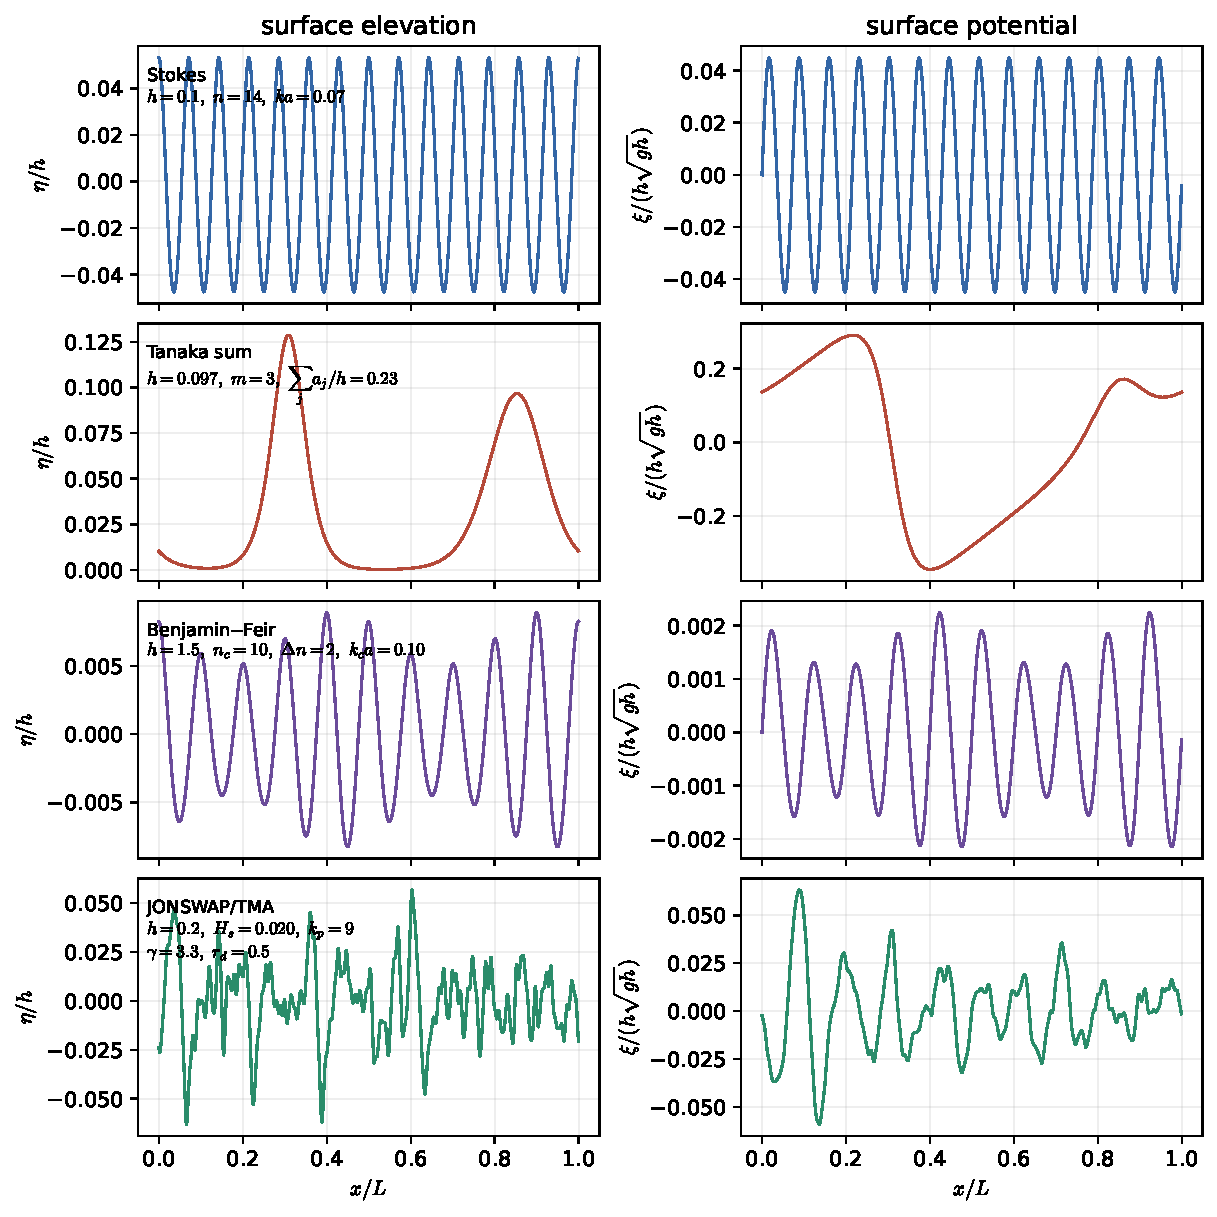
\includegraphics[width=\textwidth]{../figures/parameterized_corpus_case_examples.pdf}
  \caption{One constructed initial condition from each replacement training family.
  The columns show the dimensionless elevation $\eta/h$, surface potential
  $\xi/(h\sqrt{gh})$.  The horizontal coordinate is $x/L$, and the numerical
  plots print selected scalar descriptors in the first column.  The Stokes,
  Benjamin--Feir, and random-sea rows are generated directly from the formulas
  in this section.  The random-sea illustration uses the frozen spectral
  window that starts at wavenumber 96 and vanishes at wavenumber 128.  The Tanaka row is the fixed
  held-out case numbered 90000101 and was chosen without using model error.}
  \label{fig:training-family-examples}
\end{figure}
\FloatBarrier

Within the JONSWAP/TMA family the design gives equal case weight to its three
depth strata.  Within the other families the listed coarse strata are likewise
balanced before seeded pseudorandom sampling within each category.  In
particular, the eleven Tanaka direction-count categories are balanced as
evenly as each finite quota permits, so their counts differ by at most one.
This gives additional aggregate weight to two- and three-crest states because
they have more direction compositions.  This is a transparent
coverage design, not a claim that all categories are equally common in nature.
If $C$ is the accepted training-case count per family selected by the learning
curve, the four-family training archive contains
$C+200C+200C+16C=417C$ stored states
before any storage-level compression.  Thus the planned learning-curve grid
$C\in\{2048,4096,8192,16384\}$ corresponds to $854{,}016$ through
$6{,}832{,}128$
training rows, while retaining $4C$ accepted training-case units.  Validation,
test, and rejected attempted cases are counted separately.
The first checkpoint uses $C=2048$ training cases per family and 1024 validation
and 1024 test cases per family.  It contains exactly
$417(2048+1024+1024)=1{,}708{,}032$ retained rows.  With the current
uncompressed writer, the field archives and row map are estimated to occupy
$19.62$ GiB; the current eager loader is estimated to peak at $39.6$ GiB.
The production target is $C=16384$, with validation and test unchanged.  Its
7,686,144 rows are close to the 7,633,989 rows in historical v9: 52,155 more
rows, or 0.68\%.  The corresponding storage estimates are approximately
$88.3$ GiB of archives and row map and $178$ GiB peak memory for the eager
loader.  Thus $C=2048$ is a cumulative learning-curve checkpoint, not a
completed replacement corpus.
Rejected cases are not replaced by copying nearby accepted cases; the
attempted and accepted counts are both reported.
Using a fixed number of peak periods prevents shallow categories from facing a
much longer acceptance test merely because their dimensional time scale
differs.  The historical packet \emph{training generator} stored trajectories
to final time 120.  That archive does not set either the new packet diagnostic
horizon of 20 time units or the random-sea training horizon.


\section{Attempted and accepted counts}
\label{sec:coverage}

The tables above specify attempted populations.  For every family and every
declared parameter category, report both attempted and accepted counts.  A
category with no accepted cases is not filled from another category.  Instead, generation
stops and the support or numerical method must be revised explicitly.

The random-sea spectral window is already frozen at wavenumbers 96--128.  Its
864-case configuration audit retained at least $98.469\%$ of the reference
spectral mass in the shallow stratum and at least $99.653\%$ in the finite and
deep strata.  This is method-level evidence for the fixed constructor, not an
individual-case test.  The remaining population gate is computational:
before bulk generation, run one accepted case from
each of the 11 Tanaka, 66 Benjamin--Feir, and 27 random-sea parameter
categories with the exact contract and the bounded scheduler.  This is a
104-category trajectory pilot.

\section{Reference evolution and whole-case acceptance}
\label{sec:acceptance}

\subsection{Discrete Zakharov flow}

The reference trajectory is the solution of one declared discrete vector
field, not merely the output of the two-stage, fourth-order Gauss--Legendre
method (GL2).  The depth $h$ remains fixed.  For $w=(\eta,\xi)$, define the
internal order-six DNO evaluation and its delivered projection by
\begin{equation}
  G_{\mathrm{int}}(\eta;h)\xi
  =\G^{N,p}_M(P_K\eta;h)(P_K\xi),
  \qquad
  G_{\mathrm{ref}}(\eta;h)\xi
  =P_K^\circ\!\left[G_{\mathrm{int}}(\eta;h)\xi\right].
  \label{eq:internal-and-delivered-dno}
\end{equation}
The nonlinear product is formed with $G_{\mathrm{int}}(\eta;h)\xi$ before
the common output projection.  The discrete vector field is
\begin{equation}
  f_h(w)=
  \begin{bmatrix}
    G_{\mathrm{ref}}(\eta;h)\xi\\[2pt]
    P_K^\circ\!\left[
      -g\eta-\dfrac12\xi_x^2
      +\dfrac{\left(G_{\mathrm{int}}(\eta;h)\xi+\eta_x\xi_x\right)^2}
             {2(1+\eta_x^2)}
    \right]
  \end{bmatrix}.
\end{equation}
Let $w_0=(\eta_0,\xi_0)$ be an admissible candidate initial state, and write
$z_0=(\eta_0,\xi_0,h)$ when the fixed depth is also needed.  The reference
ODE is
\begin{equation}
  \frac{\dd w}{\dd t}=f_h(w),
  \qquad w(0)=w_0.
  \label{eq:reference-flow}
\end{equation}
The products in the second component are evaluated on the common dealiased
grid before projection.
We integrate this ODE with the GL2 scheme in the next subsection.
Removing the mean of $\partial_t\xi$ is precisely the time-dependent additive-potential
gauge; it preserves $\int_{\T_L}\xi\,\dd x=0$ without changing the velocity
field or the surface evolution.
The constructor projects both initial fields to $|k|\leq128$.  Inside every
right-hand-side evaluation, both nonlinear components are projected to that
same band, with the mean additionally removed from the $\xi$ component as in
\eqref{eq:mean-zero-band-projection}.  These projections are part of $f_h$.
After every completed GL2 step, both state components are projected once more;
that post-step projection is part of the numerical integrator rather than the
ODE vector field.

For the integrating factor, define the linear part $L_h$ and the remainder
$r_h$ by
\begin{equation}
  L_h(\eta,\xi)
  =\bigl(G_0(h)\xi,-gP_0^\perp\eta\bigr),
  \qquad
  r_h(w)=f_h(w)-L_hw.
  \label{eq:reference-linear-split}
\end{equation}
On each nonzero Fourier mode, define
$\omega_n^2=g|k_n|\tanh(h|k_n|)$.  The linear evolution is the explicit
rotation
\begin{equation}
  \begin{bmatrix}\widehat\eta_n(t)\\ \widehat\xi_n(t)\end{bmatrix}
  =
  \begin{bmatrix}
    \cos(\omega_nt) &
      \dfrac{|k_n|\tanh(h|k_n|)}{\omega_n}\sin(\omega_nt)\\[4pt]
    -\dfrac{g}{\omega_n}\sin(\omega_nt) & \cos(\omega_nt)
  \end{bmatrix}
  \begin{bmatrix}\widehat\eta_n(0)\\ \widehat\xi_n(0)\end{bmatrix}.
  \label{eq:linear-mode-evolution}
\end{equation}
The zero modes are unchanged.  We write this linear evolution as $e^{tL_h}$.
With $v(t)=e^{-tL_h}w(t)$,
\begin{equation}
  \dot v=\widetilde F(t,v)
  :=e^{-tL_h}r_h(e^{tL_h}v).
  \label{eq:integrating-factor-field}
\end{equation}

\subsection{Residual-controlled Gauss--Legendre stages}

The two-stage, fourth-order Gauss--Legendre coefficients are
\begin{equation}
  c_{1,2}=\frac12\mp\frac{\sqrt3}{6},\qquad
  A=\begin{bmatrix}
    \frac14&\frac14-\frac{\sqrt3}{6}\\[2pt]
    \frac14+\frac{\sqrt3}{6}&\frac14
  \end{bmatrix}.
  \label{eq:gl2-tableau}
\end{equation}
Let $t_n$ and $v_n$ be the current time and integrating-factor state, and
let $\delta_n>0$ be the step length.  Write $a_{ij}$ for the entries of the
matrix $A$ in \eqref{eq:gl2-tableau}.  The two stage values satisfy
\begin{equation}
  V_i=v_n+\delta_n\sum_{j=1}^{2}a_{ij}
       \widetilde F(t_n+c_j\delta_n,V_j),
  \qquad i=1,2.
  \label{eq:gl2-stages}
\end{equation}
After the stages converge,
\begin{equation}
  v_{n+1}=v_n+\frac{\delta_n}{2}
  \sum_{i=1}^2\widetilde F(t_n+c_i\delta_n,V_i).
  \label{eq:gl2-update}
\end{equation}

For a candidate pair $(V_1,V_2)$, define the fixed-point maps
\begin{equation}
  \Phi_i(V_1,V_2)
  =v_n+\delta_n\sum_{j=1}^{2}a_{ij}
       \widetilde F(t_n+c_j\delta_n,V_j),
  \qquad i=1,2.
  \label{eq:gl2-stage-map}
\end{equation}
Write $V_i^\eta,V_i^\xi$ and $\Phi_i^\eta,\Phi_i^\xi$ for their two
Fourier-space components, and let $\|\cdot\|_{\ell^2}$ be the Euclidean norm
of one component's Fourier coefficients.  The implemented relative stage
defect is
\begin{equation}
  R_n
  =
  \max_{\substack{i\in\{1,2\}\\u\in\{\eta,\xi\}}}
  \frac{\|\Phi_i^u-V_i^u\|_{\ell^2}}
       {\max\{\|\Phi_i^u\|_{\ell^2},
              \|V_i^u\|_{\ell^2},
              \operatorname{tiny}\}},
  \label{eq:gl2-residual}
\end{equation}
where $\operatorname{tiny}$ is the smallest positive normal number of the
working floating-point type.  Normalizing $\eta$ and $\xi$ separately avoids
adding fields with different units.  By Parseval's identity, the Fourier
normalization cancels from each ratio.

The stage tolerance $\tau_{\mathrm{GL}}$ and iteration cap are fixed in the
generator specification.  A stage is declared converged only when
$R_n\leq\tau_{\mathrm{GL}}$; otherwise its iteration ends at the declared cap
or when a nonfinite stage is detected.  Xu and Guyenne report that two to four
iterations typically achieved relative errors between $10^{-6}$ and
$10^{-8}$ in their applications~\cite{xu2009}; that observation motivates a
tolerance study, not an unchecked iteration count.  The implementation
recomputes \eqref{eq:gl2-residual} from the returned stages, freezes each
batched sample after convergence, and records finite cap exhaustion
separately from a nonfinite stage or state.  With
$\tau_{\mathrm{GL}}=10^{-8}$ and an eight-iteration cap, a four-code-path
$N=256$ smoke converged all 32 sampled steps in two updates.  The largest
residuals for Airy, finite Stokes, Tanaka, and the pre-revision BF
constructor were respectively
$9.08\times10^{-11}$, $1.10\times10^{-10}$,
$4.63\times10^{-10}$, and $2.09\times10^{-9}$.

\subsection{Method-level fixed-band resolution validation}

This validation is performed on a predeclared panel before production and
does not accept or reject individual corpus cases.  Resolution is tested by
reconstructing one physical specification, not by
interpolating one sampled array.  Fix a complete case record and re-evaluate
the same family formula with the same stored parameters on the three grids
$N_r=2^rN$, $r=0,1,2$.  Each reconstruction is performed independently in
float64.  Write $\eta_r$ and $\xi_r$ for the fields reconstructed on grid
$N_r$.  Define the dimensionless fields
\[
  U_r^{(\eta)}=\frac{\eta_r}{h},
  \qquad
  U_r^{(\xi)}=\frac{\xi_r}{h\sqrt{gh}},
\]
and write $\widehat U_{r,n}^{(\nu)}$ for the Fourier coefficient of
$U_r^{(\nu)}$, where $\nu\in\{\eta,\xi\}$.  The initial-state discrepancy is
\begin{equation}
  \Delta_{\mathrm{IC},K}
  =\max_{\nu\in\{\eta,\xi\}}\max_{0\leq r<s\leq2}
   \frac{
     \left(\sum_{|k_n|\leq K}
       |\widehat U_{r,n}^{(\nu)}-\widehat U_{s,n}^{(\nu)}|^2\right)^{1/2}}
        {\left(\sum_{|k_n|\leq K}|\widehat U_{s,n}^{(\nu)}|^2\right)^{1/2}
         +10^{-30}}.
  \label{eq:fixed-band-state-defect}
\end{equation}
On grid $N_r$, compute the target field
\begin{equation}
  G_r^\star=P_K^\circ\!\left[
    \G_M^{N_r,p}(P_K\eta_r;h)(P_K\xi_r)
  \right],
\end{equation}
set $U_r^{(G)}=G_r^\star/\sqrt{gh}$, and write
$\widehat U_{r,n}^{(G)}$ for its Fourier coefficients.  Then
\begin{equation}
  \Delta_{G,K}
  =\max_{0\leq r<s\leq2}
   \frac{
     \left(\sum_{|k_n|\leq K}
       |\widehat U_{r,n}^{(G)}-\widehat U_{s,n}^{(G)}|^2\right)^{1/2}}
        {\left(\sum_{|k_n|\leq K}|\widehat U_{s,n}^{(G)}|^2\right)^{1/2}
         +10^{-30}}.
  \label{eq:fixed-band-dno-defect}
\end{equation}
The frozen DNO threshold for the stratified configuration-validation panel
is $\Delta_{G,K}\leq10^{-3}$.  Both statistics are evaluated on a predeclared,
family-stratified panel before a generator revision is frozen.  A failed
panel identifies an unresolved constructor or an unsupported parameter category;
it does not authorize deleting individual production rows by inspecting
their shape.  Thus the expensive order-$M$ calculation is not repeated on
three grids at every stored time.

The historical Tanaka generator instead used a rowwise sign-transition rule.
If
$D_j=[G_{\mathrm{old}}(\eta;h)\xi](x_j)$ is the sampled old target, that rule
formed the cyclic forward difference
$d_j=(D_{j+1}-D_j)/\Delta x$, discarded entries below
$0.03\max_j|d_j|$, and rejected when the remaining cyclic sign sequence had
more than ten transitions.  It was useful for the old clipped-profile
constructor because a boundary seam generated oscillatory curvature, but a
resolved physical wave may also have many extrema.  In the completed Tanaka
calibration at the historical band $K=341$, all 12 matched clipped cases had
$\Delta_{G,K}\geq2.33\times10^{-2}$; the same specifications rebuilt by the
periodic constructor had $\Delta_{G,K}\leq1.10\times10^{-5}$, and four clean
controls had $\Delta_{G,K}\leq1.64\times10^{-4}$.  This supports the mechanism
without claiming that the current corpus was already filtered by the
three-grid statistic.  The tangent-Hermite construction removes the seam
mechanism, the three-grid panel checks its spatial resolution before
production, and production applies no sign-transition rejection.

\subsection{Method-level selection of the production time step}

Two different intervals were called \texttt{dt} in earlier project notes.
Let $\Delta s$ denote the spacing between saved states and let $\delta$ denote
the actual GL2 step in \eqref{eq:gl2-stages}--\eqref{eq:gl2-update}.  If one
saved interval is divided into $m$ equal GL2 steps, then
\begin{equation}
  \delta=\frac{\Delta s}{m}.
  \label{eq:inner-gl2-step}
\end{equation}
Production uses
\begin{equation}
  \Delta s=0.08,\qquad m=8,\qquad \delta=0.01.
  \label{eq:production-gl2-step}
\end{equation}
Thus $0.08$ is a storage interval, not the step of the GL2 method.

The choice $\delta=0.01$ was made before the present corpus plan.  The May
2026 time-step study used $m=8$ while varying the saved interval through
$\Delta s\in\{0.01,0.02,0.04,0.08,0.16,0.32\}$.  In terms of the actual GL2
step, the tested values were therefore
\[
  \delta\in\{0.00125,0.0025,0.005,0.01,0.02,0.04\}.
\]
Four Tanaka cases were integrated to $T=50$.  Relative terminal elevation
differences from the $\delta=0.00125$ calculation were about $10^{-11}$,
$10^{-10}$, and $10^{-9}$ at $\delta=0.0025$, $0.005$, and $0.01$,
respectively.  The difference jumped to $6.2\times10^{-2}$ at
$\delta=0.02$.  The historical statement ``use \texttt{dt=0.08}'' therefore
selected the largest successful \emph{saved interval with eight substeps};
it selected the actual GL2 step $\delta=0.01$, not $\delta=0.08$.

Xu and Guyenne use the same GL2 step $0.01$ in their reported
calculations~\cite{xu2009}.  Their paper does not determine our saved spacing,
residual tolerance, or complete-case policy.  Those are numerical choices
for this corpus.

The step choice was checked again in July 2026 on twelve predeclared
full-horizon cases from the trajectory families.  For this method-level
validation only, each initial condition was integrated with
$\delta=0.01$ and $0.005$ and compared at common saved times.  At a saved
time $t_j$, define
\begin{align}
  Y_\delta^{(\eta)}(t_j)&=\frac{P_K\eta_\delta(t_j)}{h},&
  Y_\delta^{(\xi)}(t_j)&=\frac{P_K\xi_\delta(t_j)}{h\sqrt{gh}},&
  Y_\delta^{(G)}(t_j)&=
    \frac{G_{\mathrm{ref}}(\eta_\delta(t_j);h)\xi_\delta(t_j)}
         {\sqrt{gh}},
  \label{eq:dimensionless-delivered-fields}
\end{align}
where $(\eta_\delta,\xi_\delta)$ is the trajectory computed with GL2 step
$\delta$.  Let $\mathcal A=\{\eta,\xi,G\}$ label the three displayed fields.
For a case specification $\theta$, the validation discrepancy was
\begin{equation}
  E(\theta;\delta)
  =
  \max_{\nu\in\mathcal A}
  \frac{
    \max_j\norm{Y_{\delta/2}^{(\nu)}(t_j)
                    -Y_\delta^{(\nu)}(t_j)}_{2,L}
  }{
    \max_j\norm{Y_{\delta/2}^{(\nu)}(t_j)}_{2,L}+10^{-12}
  }.
  \label{eq:method-refinement-error}
\end{equation}
The maximum over time in the denominator prevents a temporary cancellation
of one field from producing a large relative error.  Of the twelve cases,
ten produced complete trajectories under both steps, and all ten satisfied
\[
  E(\theta;0.01)\leq1.126337\times10^{-5}.
\]
The remaining steep Tanaka and equation-(33) Benjamin--Feir cases became
incomplete at nearly the same physical times under both steps.  Halving the
step therefore neither changed an acceptance decision nor rescued either
calculation, and no $0.0025$ calculation was needed.  Together with the May
study, this panel validates the common step $\delta=0.01$.  It does not
justify repeating the half-step calculation for every production case.
On this panel the reported integration times were $4026.06$ seconds for the
$0.01$ calculations and $7798.47$ seconds for the $0.005$ calculations.  The
pair therefore used $11824.53$ seconds of integration work, whereas the
$0.01$ arm alone used $34.0\%$ of that total.  Repeating the validation pair
in production would nearly triple the measured work of the selected method.

\subsection{Whole-case production acceptance}

Production consequently performs one rollout per attempted trajectory case,
with $\delta=0.01$, and stores candidate states every $\Delta s=0.08$.
After the initial condition has passed its declared family support, there is
one whole-trajectory acceptance condition:
\begin{quote}
The fixed numerical method must return a complete admissible trajectory on
the requested interval $[0,T]$.
\end{quote}
Here $T$ is the horizon declared by the case.  ``Complete admissible
trajectory'' means that every scheduled GL2 step reaches $T$, every implicit
stage satisfies $R_n\leq\tau_{\mathrm{GL}}=10^{-8}$, every saved state is
finite and satisfies $h+\eta>0$ on the numerical grid, and every delivered
target $G_{\mathrm{ref}}(\eta;h)\xi$ at a saved time is finite.  Failure to
reach $T$, a nonfinite field or target, an unsolved stage, and loss of the
water-wave graph domain are diagnostic causes of this one failure condition;
they are not separate fitted filters.  If the condition fails, the complete
case is rejected and no finite prefix enters the corpus.  There is no
per-case $0.005$ comparison, discrepancy threshold, or $0.0025$ retry.

For a batch of $B$ initial conditions, the production executor advances all
$B$ cases once with $\delta=0.01$.  The eight GL2 steps between consecutive
saved times are carried out inside this one batched calculation.  Random-sea
cases in the same batch can have different declared horizons.  The batch is
advanced to its longest horizon, but each case and its stage record are
restricted to that case's declared saved-time prefix before completeness and
admissibility are decided.  Values beyond a shorter case's horizon do not
belong to that case.

\begin{figure}[ht]
  \centering
  \includegraphics[width=\textwidth]
    {../../outputs/paper_corpus_current_rejection_examples_20260726/current_rejection_examples.pdf}
  \caption{Examples of the two current decisions.  In the top row, current
  finite-depth Stokes validation attempt 2 first proposes an amplitude with
  $\mathrm{Ur}_+=29.37>26$.  That amplitude is outside the declared Stokes
  support.  With the carrier, depth, phase, and steepness category unchanged, the
  next amplitude has $\mathrm{Ur}_+=20.34$ and is accepted.  Both displayed
  profiles are finite; the decision is the stated support inequality, not
  their appearance.  The middle and bottom rows use only the
  $\delta=0.01$ arms of two full-horizon validation cases that lie in their
  declared family supports.  The Tanaka trajectory has its last finite saved
  state at $t=119.44$ and first failed GL2 stage at $t=119.48$.  The
  Benjamin--Feir trajectory has its last finite saved state at $t=108.72$;
  its stage at $t=108.77$ reaches eight iterations with residual
  $3.8931\times10^{-7}>10^{-8}$.  Since both request $T=200$, the fixed
  method returns no complete trajectory and each case would contribute zero
  rows.  These are fixed validation examples, not estimates of production
  rejection probabilities.  No half-step calculation enters this figure or
  either decision.}
  \label{fig:current-rejection-examples}
\end{figure}
\FloatBarrier

Static Stokes states are not trajectories and do not use
the complete-trajectory condition.  A static case is retained only when its
declared support produces a finite state with positive water column and a
finite common target.  The three-grid, cross-family spatial audit in the
preceding subsection instead validates the constructor and common production
grid before generation; it is not a case-level filter.

The implicit stage tolerance $\tau_{\mathrm{GL}}=10^{-8}$ remains part of the
definition of the GL2 algorithm in the preceding subsection.  It specifies
when a stage equation has been solved, just as a linear-solver tolerance does;
it is not a second data-quality classifier.  Likewise, the only water-column
condition used here is the mathematical graph requirement $h+\eta>0$.  The
earlier half-depth margin $h+\eta\geq h/2$ is not part of the contract.

\subsection{Diagnostics not used for acceptance}

For grid index $\ell$, write $\eta_\ell=\eta(x_\ell)$ and
$\xi_\ell=\xi(x_\ell)$.  The monitored discrete energy is computed in
float64 using the unprojected order-$M$ DNO output evaluated from the internal
filtered state:
\begin{equation}
  \mathcal H_M^N(z)
  =\frac{\Delta x}{2}\sum_{\ell=0}^{N-1}
    \left[
      \xi_\ell\bigl(\G_M^{N,p}(\eta;h)\xi\bigr)_\ell
      +g\eta_\ell^2
    \right],
  \label{eq:discrete-hamiltonian}
\end{equation}
not reconstructed from the stored float32
$G_{\mathrm{ref}}(\eta;h)\xi=P_K^\circ[
\G_M^{N,p}(P_K\eta;h)(P_K\xi)]$ target.  Because the
implemented vector field includes spectral filtering and a truncated DNO,
$\mathcal H_M^N$ is not assumed to be an exact invariant of that discrete evolution;
its drift is a numerical diagnostic.
Let $z_n$ be the state after time step $n$, and set the fixed denominator
floor $\eps_{\mathcal H}=10^{-14}$.  The reported statistic is
\begin{equation}
  D_{\mathcal H}
  =\max_n
   \frac{|\mathcal H_M^N(z_n)-\mathcal H_M^N(z_0)|}
        {|\mathcal H_M^N(z_0)|+\eps_{\mathcal H} g h^2L}.
  \label{eq:hamiltonian-drift}
\end{equation}
It is reported on the predeclared numerical validation panels together with
mass, spectra, and stage iteration counts to validate the common numerical
method.  These quantities are not required fields in every production shard.
They do not enter case acceptance.

\subsection{Storage after acceptance}

Every requested storage time is a GL2 step endpoint: consecutive saved times
are separated by eight steps of length $0.01$.  No temporal interpolation is
used.  Stored frames are selected only
after the numerical method has returned a complete admissible trajectory, so
a failed trajectory never contributes isolated training rows.  The
production step and saved spacing are fixed by
\eqref{eq:production-gl2-step}; they are not adjusted case by case.

\section{Reference-method and surrogate validation}
\label{sec:validation}

Xu and Guyenne~\cite{xu2009} organize validation around direct DNO tests,
truncation order, dealiasing, long-time traveling waves, invariants, and time
reversal.  The replacement generator adopts the same separation of
questions.

For two states $z=(\eta,\xi,h)$ and
$\widetilde z=(\widetilde\eta,\widetilde\xi,h)$ at the same depth, define
the dimensionless state norm
\begin{equation}
  \norm{(\eta,\xi)}_h^2
  =
  \norm{\eta/h}_{2,L}^2
  +
  \norm{\xi/(h\sqrt{gh})}_{2,L}^2,
  \label{eq:dimensionless-state-norm}
\end{equation}
where the normalized spatial norm $\norm{\cdot}_{2,L}$ is defined in
\eqref{eq:l2-conventions}.  Define
their relative state error by
\begin{equation}
  \operatorname{rel}_h(z,\widetilde z)
  =\frac{\norm{(\eta-\widetilde\eta,\xi-\widetilde\xi)}_h}
         {\norm{(\widetilde\eta,\widetilde\xi)}_h+10^{-12}}.
  \label{eq:relative-state-distance}
\end{equation}
For a validation step $\delta>0$, let $z_{\delta}$ and $z_{\delta/2}$ denote
trajectories sampled at common comparison times $t_\ell$, where $\ell$
indexes those times.  Define the method-level temporal defect by
\begin{equation}
  E_t(\delta)
  =\max_\ell \operatorname{rel}_h\!\left(
    z_{\delta}(t_\ell),z_{\delta/2}(t_\ell)\right).
  \label{eq:temporal-refinement-defect}
\end{equation}
For a traveling profile, let $\sigma\in[0,L)$ denote a horizontal translation
and define
\begin{equation}
  E_{\mathrm{shape}}(t)
  =\min_{\sigma\in[0,L)}
   \frac{\norm{\eta(\cdot,t)-\eta(\cdot-\sigma,0)}_{2,L}}
        {\norm{\eta(\cdot,0)}_{2,L}+10^{-12}},
  \label{eq:translation-aligned-shape-error}
\end{equation}
and obtain the numerical displacement from the minimizing $\sigma$.
Starting from $z_0$, integrate to time $T$ and call the result
$z_{\mathrm f}$.  Starting from $z_{\mathrm f}$, use the same step
lengths in reverse order with negative sign and call the returned state
$z_{\mathrm b}$.  The forward--backward defect is
\begin{equation}
  E_{\mathrm{rev}}(T)
  =\operatorname{rel}_h(z_{\mathrm b},z_0).
  \label{eq:reversibility-defect}
\end{equation}
Thus the forward and backward calculations use exactly the same step lengths.

\begin{table}[ht]
  \centering
  \caption{Validation objects, measured quantities, and decision roles.}
  \label{tab:validation-roles}
  \small
  \begin{tabularx}{\textwidth}{
    @{}>{\raggedright\arraybackslash}p{0.20\textwidth}
       >{\raggedright\arraybackslash}X
       >{\raggedright\arraybackslash}p{0.25\textwidth}@{}}
    \toprule
    Panel & Quantity reported & Role \\
    \midrule
    Manufactured DNO
      & Exact-DNO error, discrete-target error, learned-target error, and
        end-to-end error as defined in Appendix~\ref{sec:manufactured}.
      & Selects the discrete reference configuration, not network weights. \\
    Three-grid construction
      & $\Delta_{\mathrm{IC},K}$ and $\Delta_{G,K}$ from
        \eqref{eq:fixed-band-state-defect}--\eqref{eq:fixed-band-dno-defect}.
      & Required before production; validates each constructor and the common
        spatial configuration. \\
    Time-step study
      & $E_t(\delta)$, maximum stage residual, and $D_{\mathcal H}$.
      & Required before production; selects one common GL2 step.  It is a
        method-level panel, not a calculation repeated for each corpus case. \\
    Traveling Stokes/Tanaka
      & $E_{\mathrm{shape}}(t)$, displacement divided by $t$, mass,
        \eqref{eq:hamiltonian-drift}, and $E_{\mathrm{rev}}(T)$.
      & Validates long-time propagation of the reference method. \\
    Benjamin--Feir
      & Modal amplitudes $2|\widehat\eta_n(t)|$ at the carrier and sidebands,
        recurrence error, $D_{\mathcal H}$, and high-band energy.
      & Validates modulation dynamics; growth alone is not labeled breaking. \\
    Airy
      & Flat-surface identity and cubic small-amplitude remainder scaling.
      & Post-freeze architecture verification only. \\
    Sparse Fourier
      & One-step DNO error and complete rollout error; nonfinite rollouts
        count as infinite error.
      & Development cases select only the corpus; final cases only report. \\
    Support sensitivity
      & Cellwise attempted/accepted counts under predeclared neighboring
        family-support bounds.
      & Tests whether a declared support bound removes a difficult parameter
        category; it does not alter the fixed production step. \\
    \bottomrule
  \end{tabularx}
\end{table}

Successive-$M$ differences on general states are called order sensitivity,
not convergence to the physical DNO, unless an independent boundary-integral
or conformal reference is supplied.  This qualification matters because
Xu--Guyenne report an amplitude- and resolution-dependent optimal order:
larger $M$ need not reduce error once the recursion is ill-conditioned.

The completed three-grid Tanaka study remains useful evidence that periodic
wrapping removes the old clipped-profile defect.  It does not by itself
validate the four training families, the three diagnostic suites, the time
integrator, or the choice $M=6$.

\section{Temporal sampling, splitting, and normalization}
\label{sec:splitting}

Temporal selection is performed only after the fixed-step calculation has
returned a complete admissible trajectory.  Tanaka and Benjamin--Feir trajectories are
evaluated on the dense time grid
\begin{equation}
  t_j=0.08j,\qquad j=0,\ldots,2500,
  \label{eq:adaptive-dense-times}
\end{equation}
and 200 times are retained separately for each case.  The internal GL2 step
is $0.01$; $0.08$ is the spacing of the candidate storage grid.

For Tanaka, define the discrete surface-gradient energy and its activity by
\begin{equation}
  S_{\mathrm T,j}=\sum_{\ell=0}^{N-1}
    |\partial_x\eta(x_\ell,t_j)|^2,
  \qquad
  A_{\mathrm T,j}
  =\frac{|\delta S_{\mathrm T,j}|}{S_{\mathrm T,j}+10^{-12}}.
  \label{eq:tanaka-time-activity}
\end{equation}
Here
\[
  \delta S_0=S_1-S_0,\qquad
  \delta S_j=\frac{S_{j+1}-S_{j-1}}2\ (1\leq j\leq2499),\qquad
  \delta S_{2500}=S_{2500}-S_{2499}.
\]
The derivative $\partial_x\eta$ is computed by the Fourier multiplier
$ik_n$ on the common grid.  Thus Tanaka receives extra samples
when the spatial surface derivative changes rapidly during crest interaction.

For Benjamin--Feir, define instead
\begin{equation}
  S_{\mathrm B,j}=\max_{0\leq\ell<N}|\eta(x_\ell,t_j)|,
  \qquad
  A_{\mathrm B,j}
  =\left(S_{\mathrm B,j}-\min_r S_{\mathrm B,r}\right)^4.
  \label{eq:bf-time-activity}
\end{equation}
The carrier dominates $\sum_\ell|\eta_x|^2$ and can hide the slow modulation,
so Benjamin--Feir uses the maximum absolute surface elevation rather than the
surface-gradient signal.

For either family, convolve its nonnegative activity values with a normalized
discrete Gaussian, extending the endpoint values outside the time interval.
The Gaussian standard deviation is 50 candidate-time steps for Tanaka and 20
for Benjamin--Feir; its discrete support is truncated at three standard
deviations, rounded upward to an integer number of time indices.  Call the smoothed values
$\widetilde A_{\mathrm T,j}$ and $\widetilde A_{\mathrm B,j}$.  For
$F\in\{\mathrm T,\mathrm B\}$, define
\begin{equation}
  p_{F,j}=\frac{1-\alpha_F}{2501}
    +\alpha_F\frac{\widetilde A_{F,j}}
      {\sum_{r=0}^{2500}\widetilde A_{F,r}},
  \qquad
  \alpha_{\mathrm T}=0.5,\quad \alpha_{\mathrm B}=0.85.
  \label{eq:adaptive-time-density}
\end{equation}
If the smoothed activity vanishes identically, its normalized term is replaced
by the uniform distribution.  The 200 retained indices are the deterministic
inverse-CDF locations of the midpoint quantiles
$(\ell+1/2)/200$, $\ell=0,\ldots,199$.  The first and last candidate times are
included, repeated indices are advanced to the next unused index, and all
selected indices and activity parameters are stored with the case.  This rule
depends only on the accepted reference trajectory, never on model error.

For a random-sea trajectory, let
\[
  T_{\mathrm{hor}}=16\frac{2\pi}{\omega_p},
  \qquad
  T_s=0.08\left\lfloor\frac{T_{\mathrm{hor}}}{0.08}\right\rfloor,
  \qquad
  J_s=\frac{T_s}{0.08}.
\]
It retains the saved-grid indices
\[
  j_\ell=\left\lfloor\frac{\ell J_s}{15}+\frac12\right\rfloor,
  \qquad
  t_\ell=0.08j_\ell,
  \qquad \ell=0,\ldots,15.
\]
Thus the integration ends at the last saved-grid point not exceeding sixteen
peak periods, and the retained endpoints are $0$ and $T_s$.  Static Stokes
cases retain only $t=0$, with phase already contained in the case record.

Random-sea cases in one numerical batch can have different values of $T_s$.
The single production batch is advanced to the longest required saved-grid
endpoint in the batch, but each case's fields and GL2 stage record are cropped
to its own declared prefix before completeness and admissibility are decided.
Hence values after a shorter case's horizon cannot affect its acceptance.  A
regression test obtains the same decision, retained fields, and prefix stage
record in serial and batched runs even when post-horizon values are
deliberately made nonfinite.  The all-category GPU pilot uses batch size four and
will determine whether that size is retained for production.

Training, validation, and test cases come from three disjoint tagged
PCG64 construction streams.  Their root seeds are respectively
2026072210, 2026072204, and 2026072205.
Every attempted case stores its root seed, stream identifier, and realized
parameters.  Let $s$ be the split root, let $f$ identify the physical family,
let $v$ identify the generator revision, let $r$ be the stream identifier,
and let $a$ be the attempted-case index.  Every family initializes its
per-case PCG64 stream from the five integer words $(s,f,v,r,a)$.  Thus replay
of one attempted case reproduces its complete specification without depending
on the number of earlier accepted cases.  Split membership is therefore fixed
when the attempted case specification is written, before integration or time
selection; it is not assigned from the resulting trajectory.  The training
stream continues until it has the post-acceptance count $C$ per family selected
by the learning curve.  The validation and test streams each contain 1,024
accepted cases per family, balanced over the same parameter categories to
within one case.  Every
rejected attempt remains attached to its original split manifest.
A nested training chunk is never enlarged in place.  The successive
$(C_0,A)$ pairs, where $C_0$ is the preceding cumulative count and $A$ is the
new count per family, are
\[
  (0,2048),\ (2048,2048),\ (4096,4096),\
  (8192,8192).
\]
They use distinct stream identifiers $0,1,2,3$ and the category increments in
\eqref{eq:additive-cell-quota}.  Validation and test each use one fixed,
non-nested chunk.
A requested count in one family--split category is never filled by copying or
silently drawing from another category.  In the static Stokes generator, one
candidate fixes the mode, depth, phase, and steepness category and permits at most
1000 amplitude redraws within that same category.  The sampler record contains
every rejected amplitude and its $\mathrm{Ur}_+$ value, followed by the
accepted amplitude on success.  If all 1000 redraws are exhausted, the sampler
raises with the complete strict record.  The implemented static executor
stores that record as a zero-row out-of-support attempt and schedules a
replacement in the same category.  It is not a fatal batch error.  An
unclassified error propagates without being relabeled; only the trajectory
executor's explicit fatal exception writes a terminal failure record.
This internal amplitude-redraw limit does not consume additional outer
attempts.  The replacement case does consume the next durable attempt under
\eqref{eq:cell-attempt-ceiling}.

No two temporal snapshots from the same case can appear in different
subsets.  This removes exact temporal-sibling leakage; it does not imply that
nearby parameter draws are statistically independent.

The loader implements the case-balanced rule stated in
Section~\ref{sec:dataset-design}: it selects exactly one stored time from
every accepted training case in every epoch and batches those selected rows.
The validation time for each case is fixed deterministically.  A different
number of stored times requires a separate learning-curve comparison; it is
not chosen from rollout failures.

Let $\mathcal I_{\mathrm{train}}$ denote all stored rows from accepted
training cases.  For row $i\in\mathcal I_{\mathrm{train}}$, let $\eta_i$ and
$\xi_i$ be its two input fields, let $h_i$ be its depth, and let
$G_i^\star=G_{\mathrm{ref}}(\eta_i;h_i)\xi_i$ be its target from
\eqref{eq:common-target}.  The network retains the scale normalization used by
the strongest current checkpoint, but estimates it on this set only:
\begin{equation}
  s_\eta=\max_{i\in\mathcal I_{\mathrm{train}},x}|\eta_i(x)|,
  \qquad
  s_\xi=\max_{i\in\mathcal I_{\mathrm{train}},x}|\xi_i(x)|,
  \qquad
  s_G=\max_{i\in\mathcal I_{\mathrm{train}},x}|G_i^\star(x)|.
  \label{eq:training-scales}
\end{equation}
Let $h_\star=L/(2\pi)$ be the fixed reference length.  For one row, write
$(\eta,\xi,h,G^\star)$ for its two input fields, depth, and target.  The
network receives
\begin{equation}
  \widetilde\eta=\eta/s_\eta,\qquad
  \widetilde\xi=\xi/s_\xi,\qquad
  d_h=\log\!\left(\frac{h}{h_\star}\right),\qquad
  \widetilde G^\star=G^\star/s_G.
  \label{eq:network-normalization}
\end{equation}
Hence $d_h$ is
dimensionless and is unchanged by the period rescaling in
Appendix~\ref{app:dno-rescaling}; on the production domain $L=2\pi$ it has
the same numerical value as the existing input $\log h$.
The intended corpus gives positive values for all three scales, and the
release audit verifies this before training.  The current loader nevertheless
uses one as a defensive fallback if a nonpositive scale reaches it; the
writeup does not count that fallback as validation of a malformed corpus.
No per-family, per-mode, validation, or diagnostic statistic enters
\eqref{eq:training-scales}.  The cached scales are bound to the checked
identity of the assembled dataset.
Reports include both the number of case units and the number of stored
snapshots.  Corpus size is selected by a learning curve in accepted case
count, rather than by reproducing the \texttt{v9} snapshot count by default.
The Airy, manufactured, and sparse diagnostic cases are absent from all three
training subsets and from the training-scale calculation.  If a diagnostic
result motivates a redesign, the final paper reports a fresh, case-disjoint
diagnostic draw after the revised model is frozen.

At $C$ accepted training cases per family, the case-balanced loader presents
$4C$ samples per epoch.  With global batch size 1024, comparisons at a fixed
epoch count would therefore give larger corpora more optimizer updates.  The
learning curve instead uses 10,240 optimizer updates:
\begin{center}
\begin{tabular}{@{}rrr@{}}
  \toprule
  $C$ & Steps per epoch & Epochs for 10,240 updates \\
  \midrule
  2,048  & 8   & 1,280 \\
  4,096  & 16  & 640 \\
  8,192  & 32  & 320 \\
  16,384 & 64  & 160 \\
  \bottomrule
\end{tabular}
\end{center}
The learning-rate schedule is a function of optimizer step, not epoch.
Checkpoints are compared at the same predeclared update numbers; the number
of epoch boundaries is not allowed to give the smaller corpus more
checkpoint-selection opportunities.  Test errors are first aggregated by
case within each family and then with equal weight across the four families.
A single statistic weighted by the 1, 200, 200, and 16 stored rows per case
is not a paper-level four-family result.

\section{Execution plan}
\label{sec:execution}

The target, four population laws, spatial window, reference integrator,
complete-trajectory condition, storage rule, and bounded quota mechanism are
frozen.  Before the production executor was simplified to one time step, an
exact-contract four-family smoke used run-specification schema 1 and computed
the $0.01/0.005$ validation pair:
\begin{center}
\small
\begin{tabular}{@{}lrrrr@{}}
  \toprule
  Family & Accepted & Rows & Pair discrepancy & Wall time (s) \\
  \midrule
  Stokes & 1 & 1   & ---                       & 3.782 \\
  Tanaka & 1 & 200 & $3.1953\times10^{-8}$     & 5,555.35 \\
  Benjamin--Feir & 1 & 200 & $3.7058\times10^{-8}$ & 5,561.11 \\
  JONSWAP/TMA & 1 & 16 & $7.6600\times10^{-7}$  & 835.19 \\
  \bottomrule
\end{tabular}
\end{center}
The four cases assembled into one checked dataset view containing 417 finite
rows on 1024 points, and the loader selected one time from each case.  The
pair discrepancies are method-validation evidence, and the recorded wall
times include work that production no longer performs.  The numerical target,
constructors, GL2 method, field writer, view, and loader did not change when
the attempt bound was added, but the scheduler source did.  Consequently
these run-spec-schema-1 artifacts deliberately cannot resume as a
run-spec-schema-2 run.

The eleven-category Tanaka law advances the global generator revision to 2,
and its stored parameter record uses the corresponding version-2 Tanaka
schema.  Revision-1 parameter smokes, dry runs, and all prior family pilot
artifacts remain useful as historical constructor and transaction evidence,
but they do not satisfy the revision-2 run specification and cannot be
resumed into a revision-2 run.  The 104-category trajectory gate and the
entire final corpus use revision 2.

Current generator-revision-2 numerical evidence consists of one exact case
from each of the four Stokes categories.  All four were accepted, their
quality-decision masks were zero, and the complete calculation took
$4.6875$ seconds.  The old reduced real-GL2 transactions from the trajectory
families check historical software wiring only; they are not revision-2
trajectory evidence.  The single-arm production
executor and writer pass all 31 focused acceptance, method-audit,
production-integration, writing, and quota tests; the launcher and reduced
real-GL2 smoke pass all six focused tests.  The remaining work is:

\begin{enumerate}
  \item \textbf{Complete the running all-category GPU gate.}
        This pilot is separate from the corpus and contributes no training,
        validation, or test rows.  Under the exact run-spec-schema-2 and
        generator-revision-2 contract, request
        one accepted case from each of the 11 Tanaka, 66 Benjamin--Feir, and
        27 random-sea parameter categories, using batch size four and the
        ceiling of four attempts per category.  The resulting trajectory gate
        contains 104 cases.  It passes only if every category accepts one
        case, every run is complete with no pending work or exhausted ceiling,
        all required arrays and numerical decisions are finite, every
        rejection has a decoded support reason or a diagnostic cause of an
        incomplete or inadmissible fixed-step trajectory,
        the three runs have compatible numerical and software identities, and
        wall time and peak GPU memory are recorded.

  \item \textbf{Generate the first checkpoint.}
        Generate 2048 accepted training cases and 1024 accepted validation
        and test cases from each family.  A category-ceiling failure terminates
its family run; it is not repaired by borrowing cases from another
        category.  The expected retained count is 1,708,032 rows.

  \item \textbf{Build and audit one dataset view.}
        Include all twelve completed family--split summaries, verify their
        records and file hashes, and build the row-to-case index without
        copying fields.  Check the exact family, split, case, and row counts,
        one-time-per-case training and validation selections, finite arrays,
        disjoint full case identities
        $(\text{family},\text{revision},\text{split},\text{stream},
        \text{attempt})$, and normalization scales computed only from all
        stored training rows.

  \item \textbf{Run the complete nested learning curve.}
        Extend the training split additively to
        \[
          C\in\{2048,4096,8192,16384\}
        \]
        accepted cases per family while keeping validation and test fixed.
        The final point contains 7,686,144 retained rows, comparable to
        historical v9's 7,633,989 snapshots.
        Train two seeds at every $C$ with the same architecture, optimizer,
        and 10,240-update schedule.  Compare final checkpoints at that common
        update count.  Report every point rather than stopping at an undefined
        ``material improvement'' threshold.

  \item \textbf{Test shallow mixed-mode coverage.}
        Evaluate every learning-curve endpoint on the 11 historical
        shallow-steep cases and the frozen sparse development panel.  The
        existing checkpoint C27, trained on all \texttt{v9} sources, is an
        external performance baseline, not a matched ablation.  Measure
        relative terminal elevation error and assign infinite error to every
        nonfinite rollout.  Report the median, 95th percentile, nonfinite
        count, and counts above $0.25$, $0.50$, $0.75$, and $1$.  A failure
        motivates a separately versioned population revision; it does not
        change this frozen corpus after results are seen.

  \item \textbf{Freeze and test once.}
        After all models and checkpoints are fixed, evaluate the untouched
        training-family test cases, Airy panel, manufactured-DNO panel, and
        final sparse panel.  Report errors by case within family and then
        weight the four family summaries equally.  Any later design change
        requires a new final sparse draw.
\end{enumerate}

\section{Claims this plan does and does not support}

If completed, the plan supports the following statements:
\begin{itemize}
  \item every attempted initial condition is reproducible from a complete,
        finite-dimensional case specification and one common configuration;
  \item every training label uses the same discrete operator convention;
  \item training, validation, and test rows come from disjoint cases;
  \item no Airy, manufactured-harmonic, or sparse-Fourier diagnostic row
        contributes to optimization or empirical normalization;
  \item every saved state of an accepted reference trajectory remains in the
        water-wave graph domain, and the trajectory is complete under the
        declared fixed GL2 method; and
  \item the declared four-family depth, nonlinearity, and spectral coverage is
        reported in physical dimensionless variables.
\end{itemize}

It does not, without further analysis, support the stronger statements that
the selected $G_M$ equals the physical DNO, that Hamiltonian conservation proves trajectory
accuracy, that JONSWAP spans every physically relevant sea, or that a
trajectory rejected by this numerical method is physically impossible.
Success on the four training families also does not establish arbitrary
mixed-mode generalization or accuracy below the declared shallow-TMA depth;
those remain empirical questions measured by the diagnostic suites.  The
existing C27 result cannot answer the corpus-ablation question because C27
was trained on all \texttt{v9} sources.  The order, grid, timestep, benchmark,
and new-corpus retraining studies are included precisely to keep those
questions separate.

\appendix

\section{Audit of the current \texttt{v9} archive}
\label{sec:v9}

The archive \texttt{combined\_dataset\_v9.npz} contains $7{,}633{,}989$
snapshots on $N=1024$ points over $L=2\pi$.  Its six construction categories
are Gaussian seas (460,740 rows), manufactured single modes (500,000),
fifth-order Stokes states (1,000,000), Tanaka-profile states (2,200,000),
Benjamin--Feir states (2,033,249), and sparse Fourier packets (1,440,000).
The suffixes \texttt{g0}, \texttt{g1}, and \texttt{modal} name generator runs,
not different initial-condition families or DNO orders.

The archive remains a valuable empirical baseline.  It was assembled from
generators with different row counts, filtering rules, and target
conventions.  The relevant distinctions are summarized in
Table~\ref{tab:v9-defects}.

\begin{table}[ht]
  \centering
  \caption{Why the flat \texttt{v9} archive does not define the replacement
  paper corpus.}
  \label{tab:v9-defects}
  \small
  \begin{tabularx}{\textwidth}{
    @{}>{\raggedright\arraybackslash}p{0.19\textwidth}
       >{\raggedright\arraybackslash}X
       >{\raggedright\arraybackslash}p{0.29\textwidth}@{}}
    \toprule
    Object & Current archive & Replacement rule \\
    \midrule
    Sampling rule
      & Source-dependent numbers of stored times make snapshot weight differ
        from case weight.
      & In every epoch select one stored time from every accepted case, then
        batch those selected rows. \\
    Discrete target
      & Static sources retain the direct order-six output, whereas rollout
        sources are projected to $|k|\leq128$.
      & Use \eqref{eq:common-target} for every row. \\
    Acceptance
      & Early sources were filtered rowwise; later sources used
        source-specific whole-case Hamiltonian tests.
      & Use declared support for static Stokes states and the one common
        complete fixed-step trajectory condition for the other three
        families. \\
    Reconstructibility
      & Some phase arrays and case fields were not stored, and no stage
        residual was recorded.
      & Store every parameter and test the residual
        \eqref{eq:gl2-residual}. \\
    Statistical split
      & A rowwise split can place temporal siblings in different subsets;
        normalization used the complete archive.
      & Split by attempted case and fit scales on accepted training cases. \\
    Support changes
      & Some failed parameter combinations were replaced by hand, for example
        one Benjamin--Feir mode pair.
      & Declare support first; record rejection without changing parameters. \\
    \bottomrule
  \end{tabularx}
\end{table}

Table~\ref{tab:v9-supports} records the historical parameter envelopes needed
for the direct comparison.  These are support bounds, not empirical
quantiles, and independent dimensional draws did not induce uniform density
in the dimensionless coordinates used below.  Here $H_s$ is significant wave
height, $k$ is wavenumber, $k_p$ is peak wavenumber, $k_c$ is carrier
wavenumber, $b$ is spectral bandwidth, and $n$, $n_c$, and $n_j$ are Fourier
mode indices.  The symbols $a$ and $a_j$ are wave amplitudes, $\Delta n$ is
sideband separation, and $\rho_\pm$ are sideband-to-carrier amplitude ratios.

\begin{table}[ht]
  \centering
  \caption{Historical support envelopes retained for comparison.}
  \label{tab:v9-supports}
  \small
  \begin{tabularx}{\textwidth}{
    @{}>{\raggedright\arraybackslash}p{0.18\textwidth}
       >{\raggedright\arraybackslash}X@{}}
    \toprule
    Construction & Declared support in \texttt{v9} \\
    \midrule
    Gaussian sea
      & $H_s\in[0.005,0.03]$, $k_p\in[2,12]$, bandwidth
        $b\in[1.5,5]$; $h\in[0.1,1.5]$ or $h\in[5,25]$. \\
    Manufactured mode
      & $n\in\{1,\ldots,20\}$, $h\in[0.02,1.5]$,
        $kh\in[0.02,20]$, and $0.005\leq ka\leq0.15$, subject to
        $a\in[10^{-4},0.011494]$. \\
    Stokes
      & Deep: $n\in\{1,\ldots,20\}$, $h\in[4,50]$.
        Finite: $n\in\{14,\ldots,26\}$, $h\in[0.02,1.5]$,
        $kh\in[0.5,5]$.  Both impose $ka\leq0.15$. \\
    Tanaka
      & Main: $h\in[0.01,0.30]$, one to three crests, total
        $\sum_j a_j/h\in[0.10,0.35]$.  Steep: $h\in[0.20,0.35]$,
        one crest, $a/h\in[0.25,0.45]$. \\
    Benjamin--Feir
      & $h\in[0.5,4]$, $n_c\in\{4,\ldots,20\}$,
        $k_ca\in[0.05,0.13]$, $\Delta n\in\{2,3,4\}$, and
        $\rho_\pm\in[0.05,0.20]$. \\
    Sparse Fourier
      & One to five modes, $h\in[0.005,0.5]$,
        $kh\in[0.2,1.5]$, total $a/h\in[0.03,0.25]$, and
        $\sum_j n_ja_j\leq0.15$. \\
    \bottomrule
  \end{tabularx}
\end{table}

Two historical formulas matter for interpreting the redesign.  First, the
old sea uses the following Gaussian elevation spectrum rather than the
JONSWAP/TMA construction in Section~\ref{sec:jonswap}:
\begin{equation}
  S_{\mathrm{old}}(k;k_p,b)
  =\exp\!\left[-\frac{(|k|-k_p)^2}{2(k_p/b)^2}\right].
  \label{eq:old-gaussian-spectrum}
\end{equation}
Second, the source archived as \emph{linear} is a manufactured harmonic
trace.  For wavenumber $k$, amplitude $a$, phase $\phi$, and direction sign
$s\in\{-1,1\}$, set $\vartheta=kx+\phi$ and
$\omega^2=gk\tanh(kh)$.  Then
\begin{align}
  \eta(x)&=a\cos\vartheta,\\
  \xi(x)&=s\,\frac{ag}{\omega}
    \frac{\cosh(k(h+\eta(x)))}{\cosh(kh)}\sin\vartheta.
  \label{eq:old-manufactured-xi}
\end{align}
The nonlinear dependence on $\eta$ makes this an exact manufactured
boundary trace, not a separate physical linear-wave family.

The historical depth union is approximately $0.005\leq h\leq50$.  This is
not automatically the support of the replacement dataset.  The four-family
design reaches $h\simeq0.0083$ through its shallow random-sea stratum and
$h=50$ through
Stokes; the smaller-depth interval remains diagnostic unless a separate
resolution study admits it.  The full source-by-source audit is therefore
evidence for the redesign, not the main definition of it.


\section{Diagnostic specifications and separation from training}
\label{sec:diagnostic-specifications}

The three diagnostic suites are Airy, exact manufactured, and sparse Fourier
cases.  They have complete case specifications, but they are not used for
training.  The sparse-Fourier cases are split into disjoint development and
final-test sets.
Sparse development cases may reject or revise the replacement corpus through the
predeclared gates in Section~\ref{sec:execution}; they never contribute loss
terms or normalization statistics.  Final-test cases are generated from new
case keys and remain untouched until the corpus, network, optimizer, and
checkpoint are frozen.  If a final-test result causes another design change,
it ceases to be final and another case-disjoint test draw is required.

The Airy grid is a fixed analytic verification panel, not a random
development/test draw, and is evaluated only after the network is frozen.
The manufactured panel is separate: it may select the reference
discretization $(M,N,p,K)$ because its purpose is to verify that numerical
formula, but it never selects network parameters.  No final diagnostic row
contributes to optimization, empirical normalization, network-hyperparameter
selection, or checkpoint selection.

\subsection{Airy linear-limit panel}

For the exact flat-surface test, choose an integer mode $n\geq1$, set
$k=k_n$, and choose a depth $h>0$, trace amplitude $b_{\mathrm A}>0$, and phase
$\psi\in[0,2\pi)$.  The identity is
\begin{equation}
  \eta=0,\qquad
  \xi=b_{\mathrm A}\cos(kx+\psi),\qquad
  G(0;h)\xi=k\tanh(kh)\xi.
  \label{eq:flat-dno-test}
\end{equation}
For paired phase-space tests, choose an elevation amplitude $a>0$, phase
$\phi\in[0,2\pi)$, and direction sign $s\in\{-1,1\}$.  With
$G_0(k;h)=k\tanh(kh)$ and
$\omega(k,h)=\sqrt{gG_0(k;h)}$, define
\begin{align}
  \eta_{\mathrm A}(x)&=a\cos(kx+\phi),\\
  \xi_{\mathrm A}(x)&=s\,a
  \frac{\omega(k,h)}{G_0(k;h)}\sin(kx+\phi).
  \label{eq:airy-constructor}
\end{align}
These are valid Zakharov initial data but are not asserted to be exact
nonlinear traveling waves at appreciable $ka$.  Let $\mathcal N_{\mathrm A}$
be the tested integer modes, let $\mathcal X_{\mathrm A}$ contain the tested
values of the dimensionless depth $\chi=kh$, and let
$\mathcal E_{\mathrm A}$ contain the tested values of the steepness
$\epsilon=ka$:
\begin{equation}
  \begin{aligned}
  \mathcal N_{\mathrm A}&=\{2,4,8,16,24\},\\
  \mathcal X_{\mathrm A}&=\{0.02,0.05,0.1,0.2,0.5,1,2,5,10,20\},\\
  \mathcal E_{\mathrm A}&=\{10^{-4},10^{-3},10^{-2},0.03,0.075,0.15\}.
  \end{aligned}
  \label{eq:airy-diagnostic-grid}
\end{equation}
For every $n\in\mathcal N_{\mathrm A}$, $\chi\in\mathcal X_{\mathrm A}$,
and $\epsilon\in\mathcal E_{\mathrm A}$, set
\begin{equation}
  k_n=\frac{2\pi n}{L},\qquad h=\frac{\chi}{k_n},\qquad
  a=\frac{\epsilon}{k_n},
\end{equation}
and retain only categories satisfying
\begin{equation}
  0.005\leq h\leq50,\qquad
  \frac{a}{h}=\frac{\epsilon}{\chi}\leq0.16.
  \label{eq:airy-feasibility}
\end{equation}
Use both $s=\pm1$ and phases $\phi\in\{0,\sqrt2\}$ radians; the latter are
not related by an integer-grid shift on the $N=1024$ grid.  The flat test
uses the same $(n,\chi)$ categories, $\psi\in\{0,\sqrt2\}$, and
$b_{\mathrm A}\in\{10^{-3},10^{-2},10^{-1}\}$.  These rules determine
$(n,h,a,\phi,s)$ or $(n,h,b_{\mathrm A},\psi)$ completely and exclude
bottom-crossing surfaces.

The amplitude ladder tests the declared small-surface structure of the
\emph{discrete target}; no independent nonlinear physical-DNO solver is
assumed here.  Define
\begin{align}
  r_{\mathrm A}^{\star}(a)
  ={}&G_{\mathrm{ref}}(\eta_{\mathrm A};h)\xi_{\mathrm A}\notag\\
   &-P_K^\circ\!\left[
      G_0(h)P_K\xi_{\mathrm A}
      +G_1(P_K\eta_{\mathrm A};h)P_K\xi_{\mathrm A}
    \right].
  \label{eq:airy-discrete-remainder}
\end{align}
Both $\eta_{\mathrm A}$ and $\xi_{\mathrm A}$ are proportional to $a$.
Therefore $G_0(h)\xi_{\mathrm A}$ has degree one in $a$,
$G_1(\eta_{\mathrm A};h)\xi_{\mathrm A}$ has degree two, and
$G_m(\eta_{\mathrm A};h)\xi_{\mathrm A}$ has degree $m+1$.  After subtracting
the first two terms, the remainder therefore begins at degree three:
\begin{equation}
  \norm{r_{\mathrm A}^{\star}(a)}_{2,L}=O(a^3)
  \qquad(a\to0)
  \label{eq:airy-remainder-scaling}
\end{equation}
at fixed $(k,h,\phi,s)$ and fixed $(M,N,p,K)$.  When the projected $G_2$
coefficient is nonzero, the predicted leading slope is three; a vanishing
coefficient is reported rather than fitted on roundoff.  The diagnostic is
the least-squares slope of $\log\norm{r_{\mathrm A}^{\star}(a)}_{2,L}$
against $\log a$ over the three smallest usable amplitudes.  The learned
remainder is defined by replacing $G_{\mathrm{ref}}(\eta_{\mathrm A};h)
\xi_{\mathrm A}$ with the network output.
Thus the flat-surface identity is a physical analytic test, whereas the
nonlinear amplitude ladder tests consistency with the declared polynomial
target and architecture.
Thus this held-out panel is more informative about the analytic
$G_0+G_1+O(\eta^2)$ architecture than a large collection of similar
single-mode training rows.

\subsection{Manufactured exact-DNO panel}
\label{sec:manufactured}

For an integer mode $n\geq1$, set $k=k_n$.  Choose a depth $h>0$, amplitude
$a>0$, phase $\phi\in[0,2\pi)$, and direction sign $s\in\{-1,1\}$, and set
$\omega=\omega(k,h)=\sqrt{gk\tanh(kh)}$.  Define
\begin{equation}
  \varphi(x,y)
  =s\,\frac{ag}{\omega}
    \frac{\cosh(k(y+h))}{\cosh(kh)}\sin(kx+\phi),\qquad
  \eta(x)=a\cos(kx+\phi).
  \label{eq:manufactured-potential}
\end{equation}
The boundary trace is exactly \eqref{eq:old-manufactured-xi}, and the normal
derivative is known without solving a boundary-value problem:
\begin{equation}
  [G_{\mathrm{exact}}(\eta;h)\xi](x)
  =\left(\varphi_y-\eta_x\varphi_x\right)_{y=\eta(x)}.
  \label{eq:manufactured-exact-dno}
\end{equation}
This is the one-dimensional counterpart of the direct DNO test in
Xu--Guyenne equations (30)--(32)~\cite{xu2009}.  For the exact benchmark, the
full trace $\xi=\varphi|_{y=\eta}$ is evaluated on a sufficiently resolved
grid and the unprojected $\G^{N,p}_M(\eta;h)\xi$ is compared with
$G_{\mathrm{exact}}(\eta;h)\xi$.  This is distinct from the training target
\eqref{eq:common-target}: in general
\begin{equation}
  G(\eta;h)(P_K\xi)\neq G(\eta;h)\xi.
\end{equation}
The frozen manufactured grid uses the same
$n\in\mathcal N_{\mathrm A}$, $kh\in\mathcal X_{\mathrm A}$,
$ka\in\mathcal E_{\mathrm A}$, feasibility condition
\eqref{eq:airy-feasibility}, phases $\phi\in\{0,\sqrt2\}$, and signs
$s=\pm1$ as the Airy panel.  The constructor
\eqref{eq:manufactured-potential} then determines the full boundary trace and
exact normal derivative, so every benchmark case is reconstructible.

Once the reference configuration is frozen, let $G_{\mathrm{net}}$ denote
the frozen learned surrogate.  Report four different errors:
\begin{align}
  e_{\mathrm{CS}}
  &=\frac{\norm{\G^{N,p}_M(\eta;h)\xi-
                   G_{\mathrm{exact}}(\eta;h)\xi}_2}
          {\norm{G_{\mathrm{exact}}(\eta;h)\xi}_2},\\
  e_{\mathrm{target}}
  &=\frac{\norm{G_{\mathrm{ref}}(\eta;h)\xi-
                   P_K^\circ[G_{\mathrm{exact}}(\eta;h)\xi]}_2}
          {\norm{P_K^\circ[G_{\mathrm{exact}}(\eta;h)\xi]}_2},\\
  e_{\mathrm{learn}}
  &=\frac{\norm{G_{\mathrm{net}}(P_K\eta;h)(P_K\xi)-
                   G_{\mathrm{ref}}(\eta;h)\xi}_2}
          {\norm{G_{\mathrm{ref}}(\eta;h)\xi}_2},\\
  e_{\mathrm{total},K}
  &=\frac{\norm{G_{\mathrm{net}}(P_K\eta;h)(P_K\xi)-
                   P_K^\circ[G_{\mathrm{exact}}(\eta;h)\xi]}_2}
          {\norm{P_K^\circ[G_{\mathrm{exact}}(\eta;h)\xi]}_2}.
  \label{eq:manufactured-error-split}
\end{align}
Here $e_{\mathrm{CS}}$ measures the unprojected order-$M$ reference,
$e_{\mathrm{target}}$ is the total discrepancy of the declared discrete
target and therefore combines Craig--Sulem, grid, input-projection, and
output-projection effects; it is not an isolated projection error.
$e_{\mathrm{learn}}$ isolates fitting of the declared discrete target, and
$e_{\mathrm{total},K}$ is the end-to-end fixed-band error.  This
prevents reference truncation or projection error from being credited to or
blamed on the network.

\subsection{Sparse-Fourier shallow stress suite}

These cases test shallow mixed-mode generalization and are never used for
training.  Choose a depth \(h>0\), a mode count \(m\in\{2,3,4,5\}\), and
distinct positive Fourier indices \(n_1,\ldots,n_m\).  For each component,
choose an amplitude \(a_j>0\), phase \(\phi_j\in[0,2\pi)\), and direction
\(s_j\in\{-1,1\}\).  The initial state is
\begin{align}
  \eta_{\mathrm F}(x)&=\sum_{j=1}^{m}a_j\cos(k_{n_j}x+\phi_j),\\
  \xi_{\mathrm F}(x)&=\sum_{j=1}^{m}s_j a_j
       \frac{\omega(k_{n_j},h)}{G_0(k_{n_j};h)}
       \sin(k_{n_j}x+\phi_j).
  \label{eq:fourier-packet}
\end{align}
Here \(G_0(k;h)=k\tanh(kh)\) and
\(\omega(k,h)=\sqrt{gG_0(k;h)}\), as in the Airy construction.  Fresh cases
satisfy
\begin{equation}
  0.02\leq h\leq0.12,\qquad
  0.2\leq k_{n_j}h\leq1.5,\qquad
  0.03\leq\sum_{j=1}^{m}\frac{a_j}{h}\leq0.18,\qquad
  \sum_{j=1}^{m}k_{n_j}a_j\leq0.15.
  \label{eq:fourier-support}
\end{equation}

Each fresh panel contains 256 attempted cases.  Divide the depth interval
logarithmically into four parts, divide the allowed total amplitude
\(\sum_j a_j/h\) into a lower and an upper half, and distinguish
unidirectional cases, in which all \(s_j\) agree, from bidirectional cases,
in which both signs occur.  Attempt four cases in every combination of the
four depth intervals, four mode counts, two amplitude halves, and two
direction classes.  A deterministic seeded PCG64 stream selects the remaining
continuous quantities within each category.  The stream identifier and all modes,
amplitudes, phases, directions, case indices, and realized parameters are
stored.

The development and final panels use the respective seeds 2026072201 and
2026072202.  Rejection never causes replacement.  At least two of the four
attempts in every category must pass the common reference checks; otherwise the
panel construction fails.  The final panel remains untouched until the
corpus, model, optimizer, and checkpoint rule are frozen.

The 11 historical shallow initial conditions are also retained as a separate
development panel, but their trajectories are recomputed with the same frozen
reference solver used everywhere else; the old trajectory files are
historical evidence only.  All sparse-Fourier rollouts have final time 20 and
are stored every 0.08 time units.  An earlier unmatched comparison suggested
that shallow packets reduced the shallow error tail, but simultaneous changes
in corpus size, normalization, and device count prevent a causal claim.  That
observation motivates this held-out test, not a sparse-Fourier training
family.
\section{Rescaling to the \texorpdfstring{$2\pi$}{2pi} reference torus}
\label{app:dno-rescaling}

The period dependence of $G$ is suppressed in
\eqref{eq:physical-dno}.  In this appendix only, write
$G^{[L]}(\eta;h)$ for the physical DNO on $\T_L$.  Set
$\lambda=L/(2\pi)$ and write $x=\lambda X$, $y=\lambda Y$.  Define
\begin{equation}
  \bar\eta(X)=\frac{\eta(\lambda X)}{\lambda},
  \qquad
  \bar\xi(X)=\xi(\lambda X),
  \qquad
  \bar h=\frac{h}{\lambda}.
  \label{eq:rescaled-dno-data}
\end{equation}
\begin{equation}
  \boxed{
  [G^{[L]}(\eta;h)\xi](\lambda X)
  =\frac1\lambda
   [G^{[2\pi]}(\bar\eta;\bar h)\bar\xi](X).
  }
  \label{eq:dno-period-rescaling}
\end{equation}
Indeed, $\bar\varphi(X,Y)=\varphi(\lambda X,\lambda Y)$ solves the same
Laplace--Neumann--Dirichlet problem below $\bar\eta$ at depth $\bar h$.
The chain rule gives $\bar\varphi_X=\lambda\varphi_x$,
$\bar\varphi_Y=\lambda\varphi_y$, and
$\bar\eta_X(X)=\eta_x(\lambda X)$, which proves
\eqref{eq:dno-period-rescaling} directly.

The cutoff in this document is a physical wavenumber cutoff.  Let
$P_K^{[L]}$ denote projection on $\T_L$ onto integer Fourier indices
$j\in\mathbb Z$ satisfying $|2\pi j/L|\leq K$, and
let $P_{\lambda K}^{[2\pi]}$ denote the corresponding projection on
$\T_{2\pi}$.  For $\bar f(X)=f(\lambda X)$,
\begin{equation}
  (P_K^{[L]}f)(\lambda X)
  =P_{\lambda K}^{[2\pi]}\bar f(X).
  \label{eq:projection-period-rescaling}
\end{equation}
Write $G_{\mathrm{ref},K}^{[L]}$ for the operator in
\eqref{eq:common-target} evaluated on $\T_L$ with cutoff $K$, and write
$G_{\mathrm{ref},\lambda K}^{[2\pi]}$ for the corresponding operator on
$\T_{2\pi}$.  If the same Fourier indices are present on both $N$-point
grids, then, up to floating-point roundoff,
\begin{equation}
  \boxed{
  \lambda
  [G_{\mathrm{ref},K}^{[L]}(\eta;h)\xi](\lambda X)
  =
  [G_{\mathrm{ref},\lambda K}^{[2\pi]}
    (\bar\eta;\bar h)\bar\xi](X).
  }
  \label{eq:discrete-period-rescaling}
\end{equation}

For Fourier index $j$, $k_j=2\pi j/L=j/\lambda$, whereas the corresponding
reference-torus wavenumber is $\bar k_j=j$.  Define
$\bar a=a/\lambda$, $\bar H_s=H_s/\lambda$, and
$\bar k_p=\lambda k_p$.  Then
$k_jh=\bar k_j\bar h$, $k_ja=\bar k_j\bar a$,
$a/h=\bar a/\bar h$, $H_s/(2h)=\bar H_s/(2\bar h)$, and
$k_pH_s/2=\bar k_p\bar H_s/2$.  Thus each dimensionless combination used in
the family definitions is unchanged by a uniform rescaling of length.

The production corpus remains on $L=2\pi$.  Equations
\eqref{eq:dno-period-rescaling}--\eqref{eq:discrete-period-rescaling} are
pre-normalization identities for DNO evaluation; they do not by themselves
define a variable-period training augmentation.  A full trajectory
rescaling at fixed gravity uses $\tau=t/\sqrt{\lambda}$.  The rescaled fields
are
\[
  \eta^\sharp(X,\tau)
    =\lambda^{-1}\eta(\lambda X,\sqrt\lambda\,\tau),\qquad
  \xi^\sharp(X,\tau)
    =\lambda^{-3/2}\xi(\lambda X,\sqrt\lambda\,\tau),
\]
\[
  [G^{[2\pi]}(\eta^\sharp(\cdot,\tau);\bar h)
       \xi^\sharp(\cdot,\tau)](X)
  =\lambda^{-1/2}
    [G^{[L]}(\eta(\cdot,\sqrt\lambda\,\tau);h)
       \xi(\cdot,\sqrt\lambda\,\tau)](\lambda X).
\]
It must therefore be treated as a separate change of variables rather than
an archive-level spatial resize.

\begin{thebibliography}{9}

\bibitem{zhao2022}
K.~Zhao and P.~L.-F.~Liu,
\newblock On Stokes wave solutions,
\newblock \emph{Proceedings of the Royal Society A} 478 (2022), 20210732,
\href{https://doi.org/10.1098/rspa.2021.0732}
{doi:10.1098/rspa.2021.0732}.

\bibitem{fenton1985}
J.~D.~Fenton,
\newblock A fifth-order Stokes theory for steady waves,
\newblock \emph{Journal of Waterway, Port, Coastal, and Ocean Engineering}
111(2) (1985), 216--234,
\href{https://doi.org/10.1061/(ASCE)0733-950X(1985)111:2(216)}
{doi:10.1061/(ASCE)0733-950X(1985)111:2(216)}.

\bibitem{zhao2024}
K.~Zhao, Y.~Wang, and P.~L.-F.~Liu,
\newblock A guide for selecting periodic water wave theories:
Le M\'ehaut\'e (1976)'s graph revisited,
\newblock \emph{Coastal Engineering} 188 (2024), 104432,
\href{https://doi.org/10.1016/j.coastaleng.2023.104432}
{doi:10.1016/j.coastaleng.2023.104432}.

\bibitem{xu2009}
L.~Xu and P.~Guyenne,
\newblock Numerical simulation of three-dimensional nonlinear water waves,
\newblock \emph{Journal of Computational Physics} 228 (2009), 8446--8466,
\href{https://doi.org/10.1016/j.jcp.2009.08.015}
{doi:10.1016/j.jcp.2009.08.015}.

\bibitem{tanaka1986}
M.~Tanaka,
\newblock The stability of solitary waves,
\newblock \emph{The Physics of Fluids} 29(3) (1986), 650--655,
\href{https://doi.org/10.1063/1.865459}
{doi:10.1063/1.865459}.

\bibitem{benjaminfeir1967}
T.~B.~Benjamin and J.~E.~Feir,
\newblock The disintegration of wave trains on deep water. Part 1. Theory,
\newblock \emph{Journal of Fluid Mechanics} 27(3) (1967), 417--430,
\href{https://doi.org/10.1017/S002211206700045X}
{doi:10.1017/S002211206700045X}.

\bibitem{dommermuth1987}
D.~G.~Dommermuth and D.~K.~P.~Yue,
\newblock A high-order spectral method for the study of nonlinear gravity
waves,
\newblock \emph{Journal of Fluid Mechanics} 184 (1987), 267--288,
\href{https://doi.org/10.1017/S002211208700288X}
{doi:10.1017/S002211208700288X}.

\bibitem{hasselmann1973}
K.~Hasselmann et al.,
\newblock Measurements of wind-wave growth and swell decay during the Joint
North Sea Wave Project (JONSWAP),
\newblock \emph{Erg\"anzungsheft zur Deutschen Hydrographischen Zeitschrift},
Reihe A(8), No.~12, 1973.

\bibitem{bouws1985}
E.~Bouws, H.~G\"unther, W.~Rosenthal, and C.~L.~Vincent,
\newblock Similarity of the wind wave spectrum in finite depth water:
1. Spectral form,
\newblock \emph{Journal of Geophysical Research: Oceans} 90(C1) (1985),
975--986,
\href{https://doi.org/10.1029/JC090iC01p00975}
{doi:10.1029/JC090iC01p00975}.

\end{thebibliography}

\end{document}
